% !TEX root = ../main.tex

\chapter{Temporal prediction of multiple sclerosis evolution from patient-centered outcomes} \label{chap:aism}
% AISM

\begin{displayquote}
%	This chapter describes a patient-centered outcomes-based ML model that predicts the disease evolution of multiple sclerosis patients.
	In this chapter, we investigate on
	use of patient-centered outcomes to predict the evolution of multiple sclerosis and to assess its impact on patients' lives.
	Multiple Sclerosis is a degenerative condition of the central nervous system that affects nearly $2.5$ million of individuals in terms of their physical, cognitive, psychological and social capabilities. Despite the high variability of its clinical presentation, \textit{relapsing} and \textit{progressive} multiple sclerosis are considered the two main disease types, with the former possibly evolving into the latter.
	%Nowadays no acknowledged clinical tests to diagnose multiple sclerosis or to distinguish between its types have been proposed.
	Recently, the attention of the medical community toward the use of patient-centered outcomes in multiple sclerosis has significantly increased. Such patient-friendly measures are devoted to the assessment of the impact of the disease on several domains of the patient life.
	% One of the open questions in the field is the use of patient-centered outcomes to assess multiple sclerosis impact on patients' lives and to predict the evolution of the disease.
	%To date, a clear understanding on whether it is possible to define a predictive model based on them is still an open question.
	%the use of such measures to assess neurodegenerative diseases evolution is still lacking. Moreover,
	To this aim, we build a novel temporal model based on gradient boosting classification and multiple-output elastic-net regression. The model
	%  is entirely based on patient-centered outcomes and it
	provides clinically interpretable results along with accurate predictions of the disease course evolution.
\end{displayquote}

\section{Introduction: the evolution of multiple sclerosis} \label{sec:aism_intro}

Multiple Sclerosis (MS) is a neurodegenerative and chronic disease of the central nervous system characterized by damages to the myelin sheaths, resulting in a wide range of symptoms, such as fatigue, numbness, visual disturbances, bladder problems, mobility issues and cognitive deficits.

% \todo{In clinical practice, accurate patient evaluation and clinical judgement remain the basics in MS diagnosis, as the identification of a validated set of biomarkers is still an open problem~\cite{milo2014revised}.}

People with MS (PwMS) are mainly classified according to their disease course:
relapsing-remitting (\ac{RR}), secondary-progressive (\ac{SP}), primary-progressive (\ac{PP}) and progressive-relapsing (\ac{PR})~\cite{giovannoni2016brain} and benign (\ac{B}).
Neurological disability in \RR patients is mainly due to the development of multifocal inflammatory lesions and it results in relapses, that are attacks of neurological worsening (\ie \textit{relapses}), followed by partial or complete recovery. Disability accrues predominantly in progressive courses (\SP, \PP, \PR) that are more characterized from diffuse immune mechanisms and neurodegeneration.
Benign MS occurs when the patient remains fully functional in all neurologic systems for at least $15$ years after the onset.
Figure~\ref{fig:ms_mock} shows a representative disability progression of MS patients according to their disease course.

An estimated $15\%$ of PwMS have a \PP or \PR course at the onset, the remaining $85\%$ is diagnosed with a \RR course.
About $80\%$ of \RR patients develop \SP course within $15\text{--}20$ years if untreated, or if the adopted pharmacological and rehabilitative protocols are not continuously adjusted according to the evolution of the disease~\cite{scalfari2014onset}.

\begin{figure}[]
	\centering
	\subfloat[]{%
		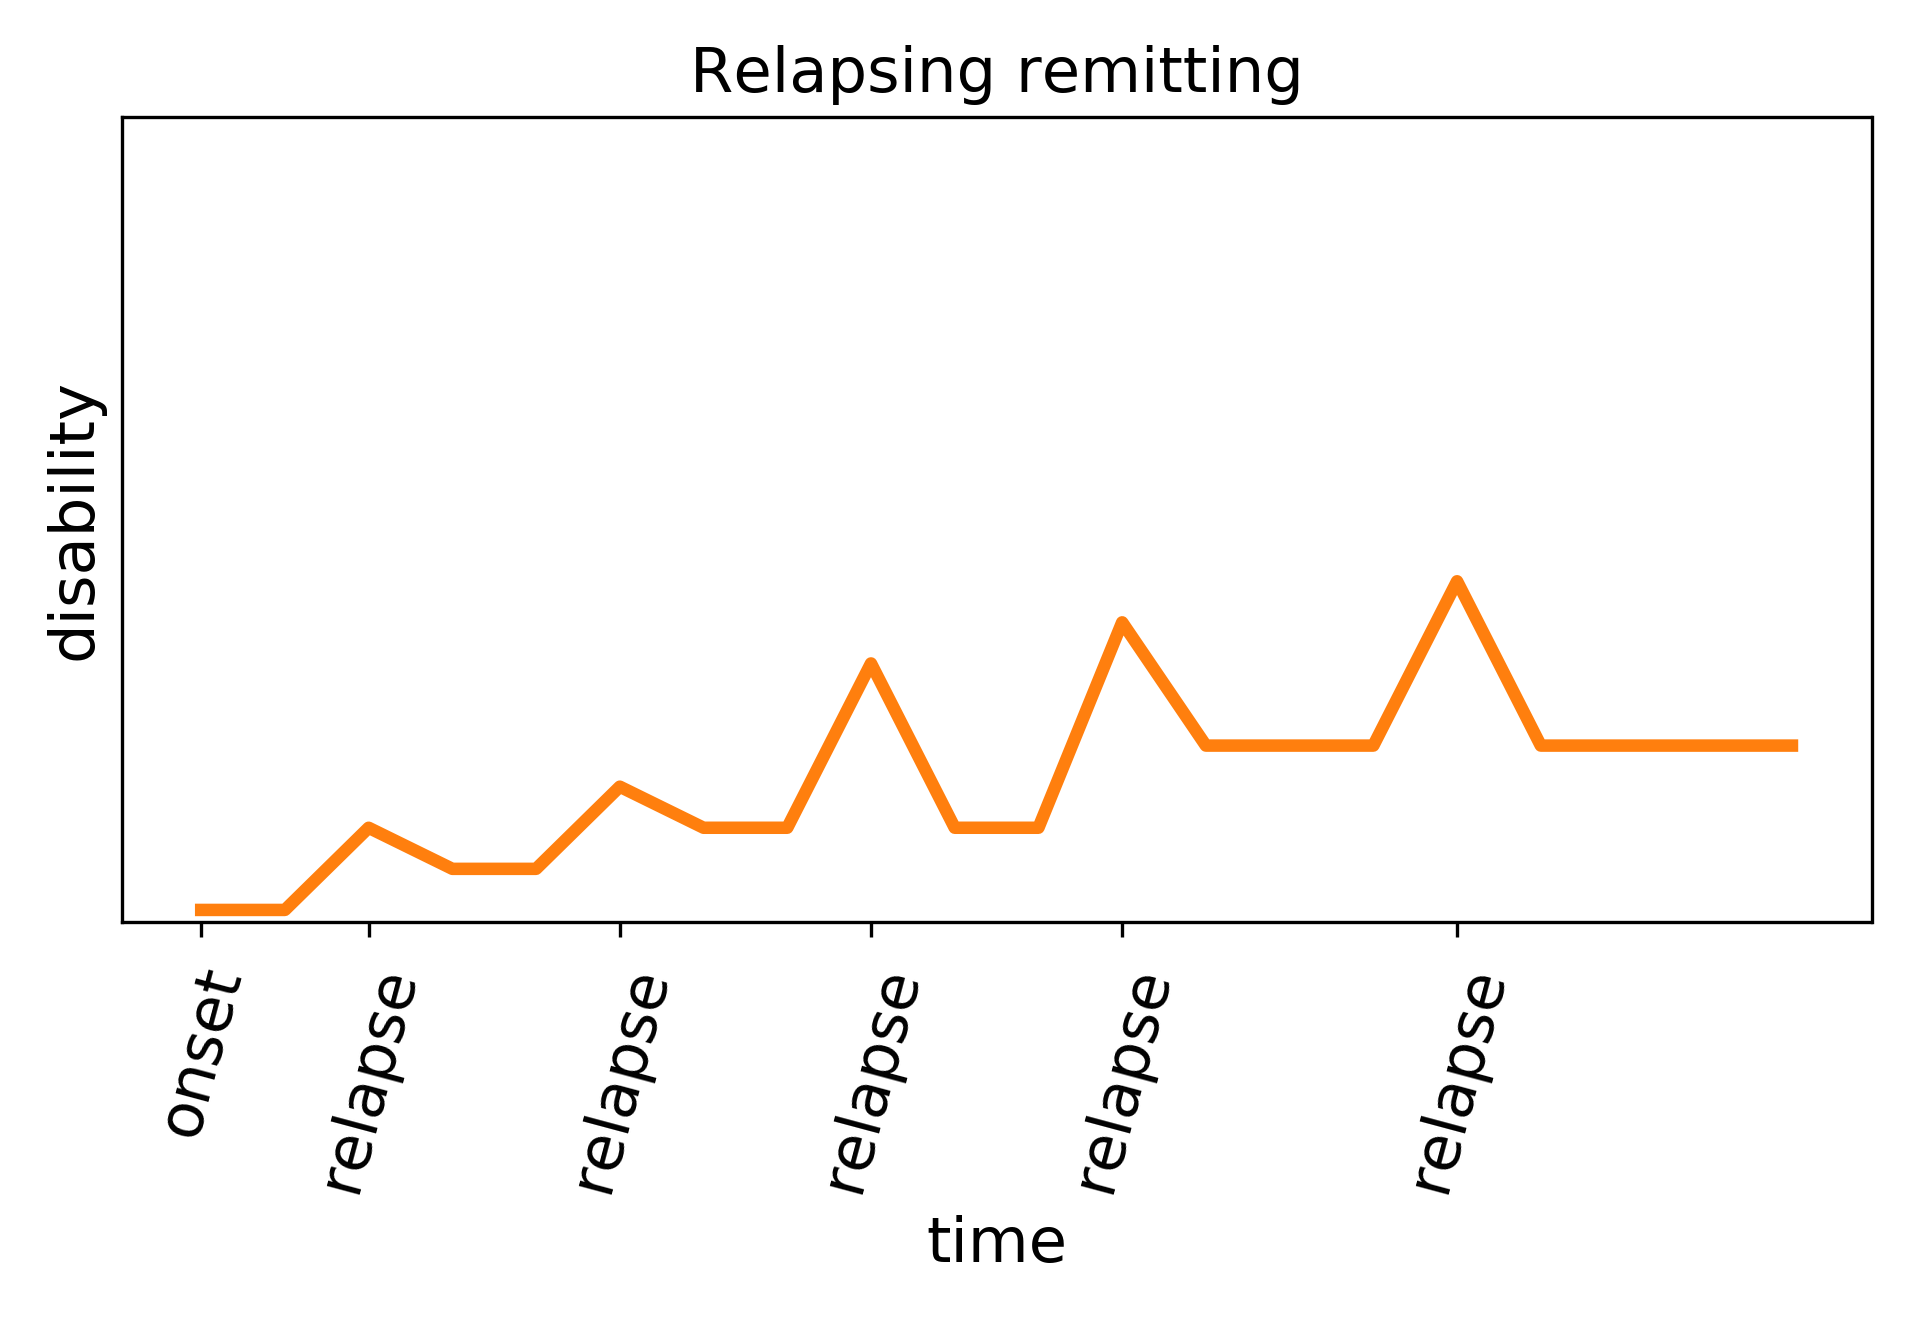
\includegraphics[width=0.5\textwidth]{part2/ms_mock_rr.png}
		\label{fig:ms_mock_rr}%
	}%
	\subfloat[]{%
		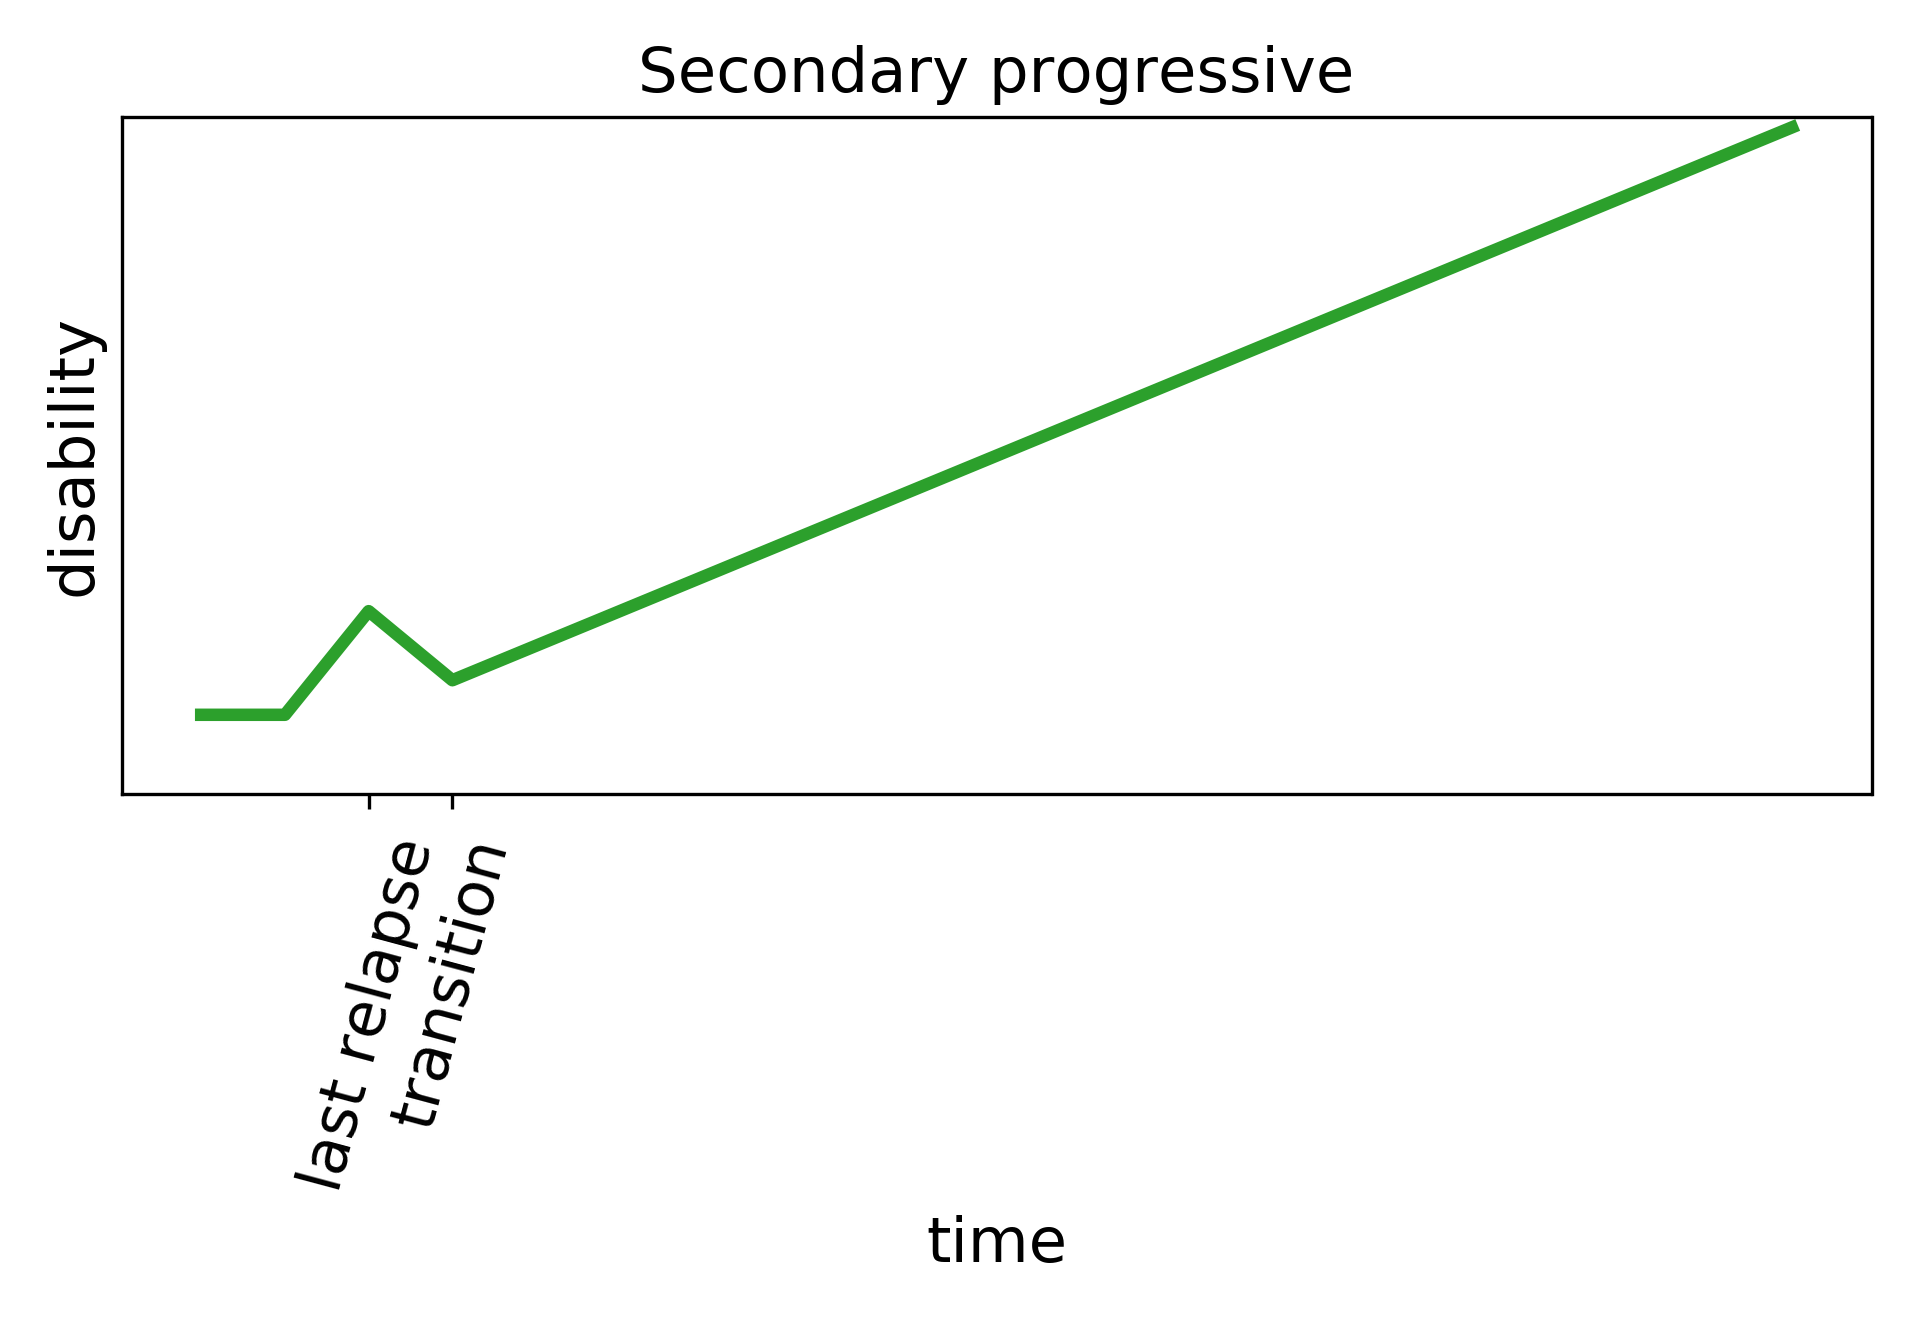
\includegraphics[width=0.5\textwidth]{part2/ms_mock_sp.png}
		\label{fig:ms_mock_sp}%
	}
	\hfill
	\subfloat[]{%
		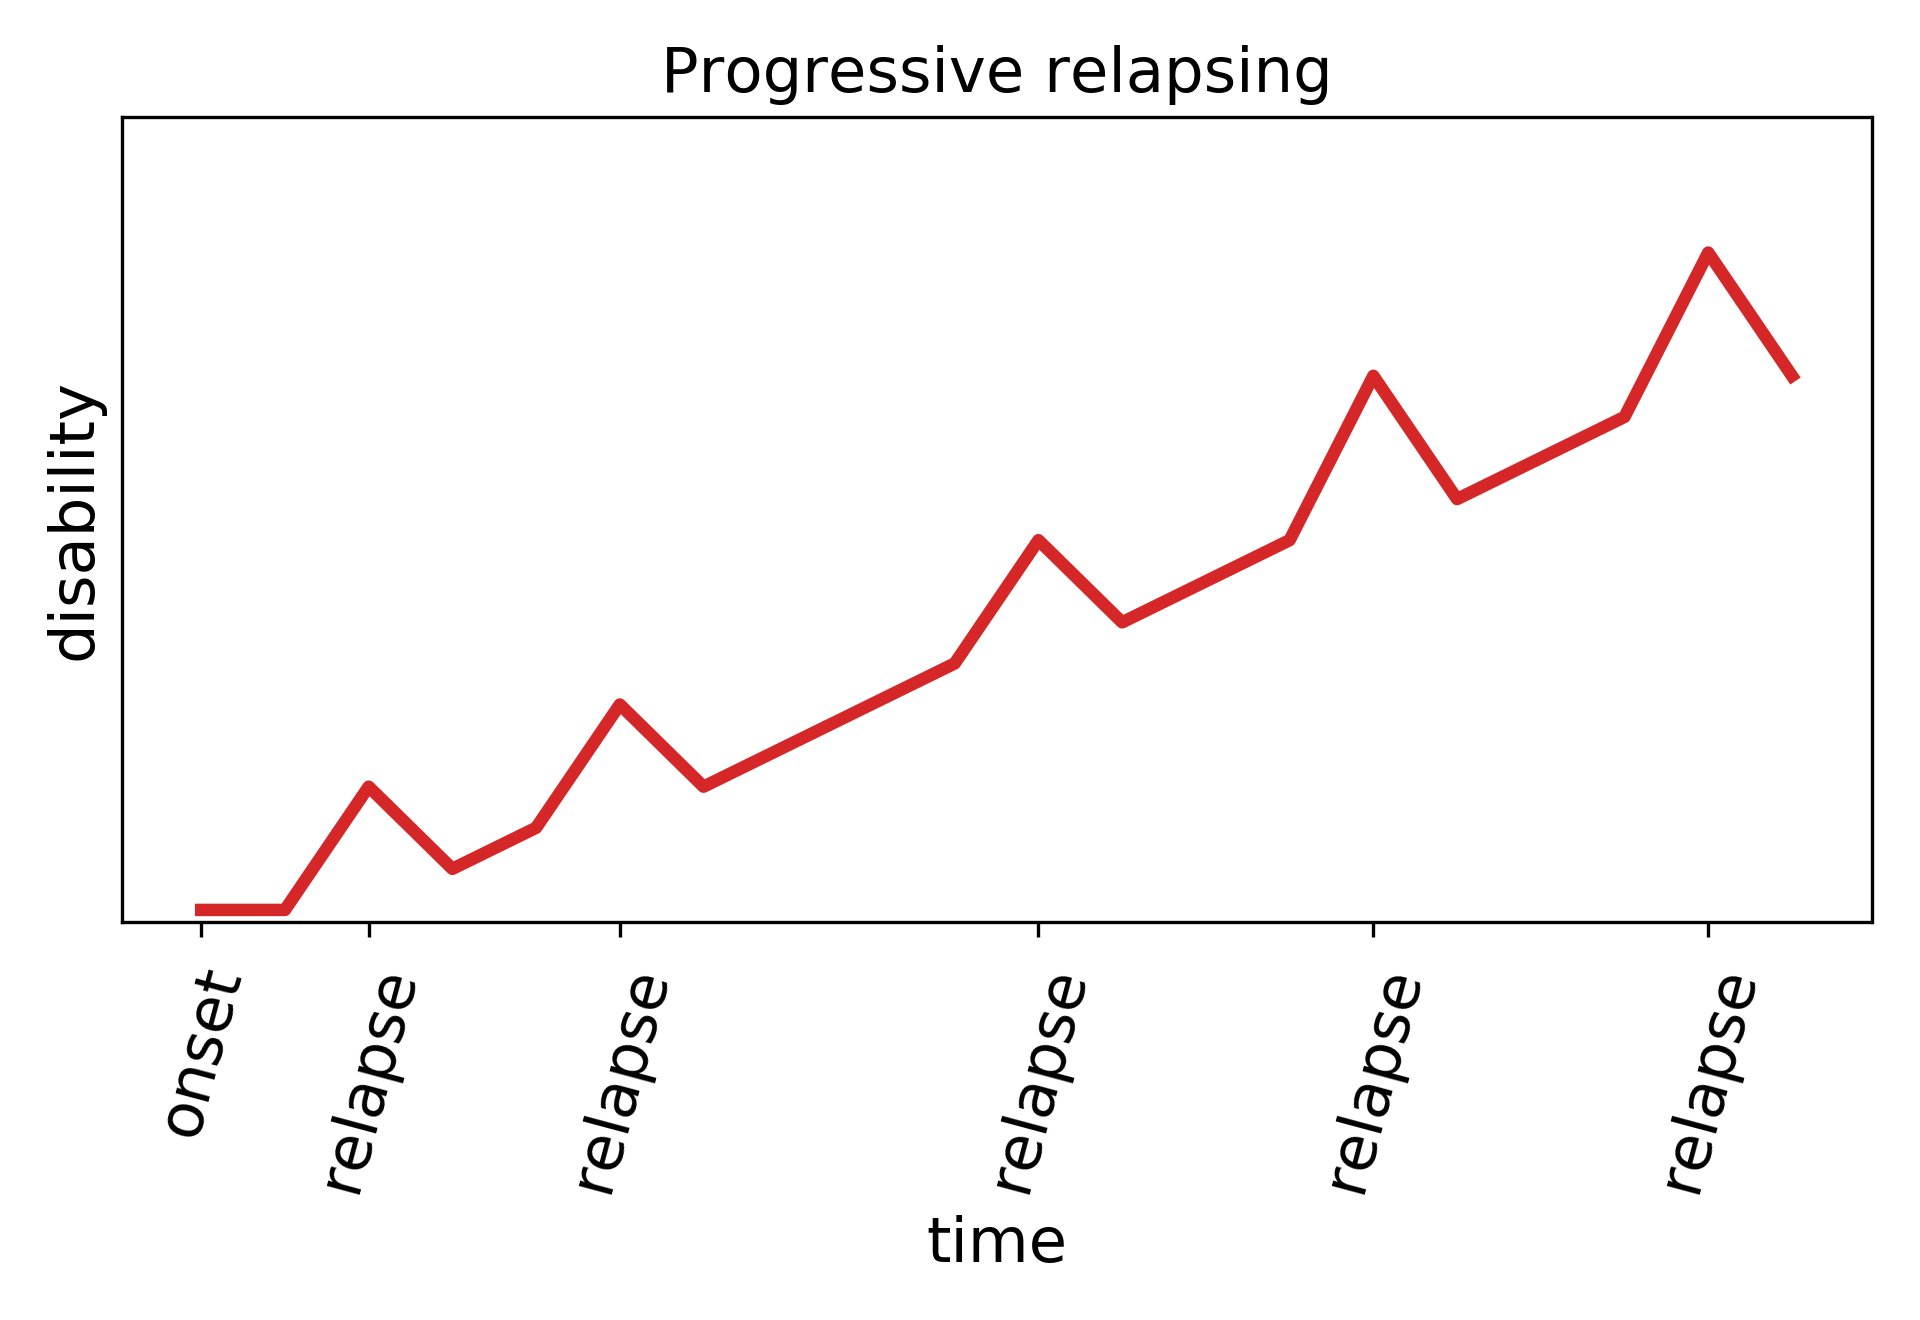
\includegraphics[width=0.5\textwidth]{part2/ms_mock_pr.png}
		\label{fig:ms_mock_pr}%
	}%
	\subfloat[]{%
		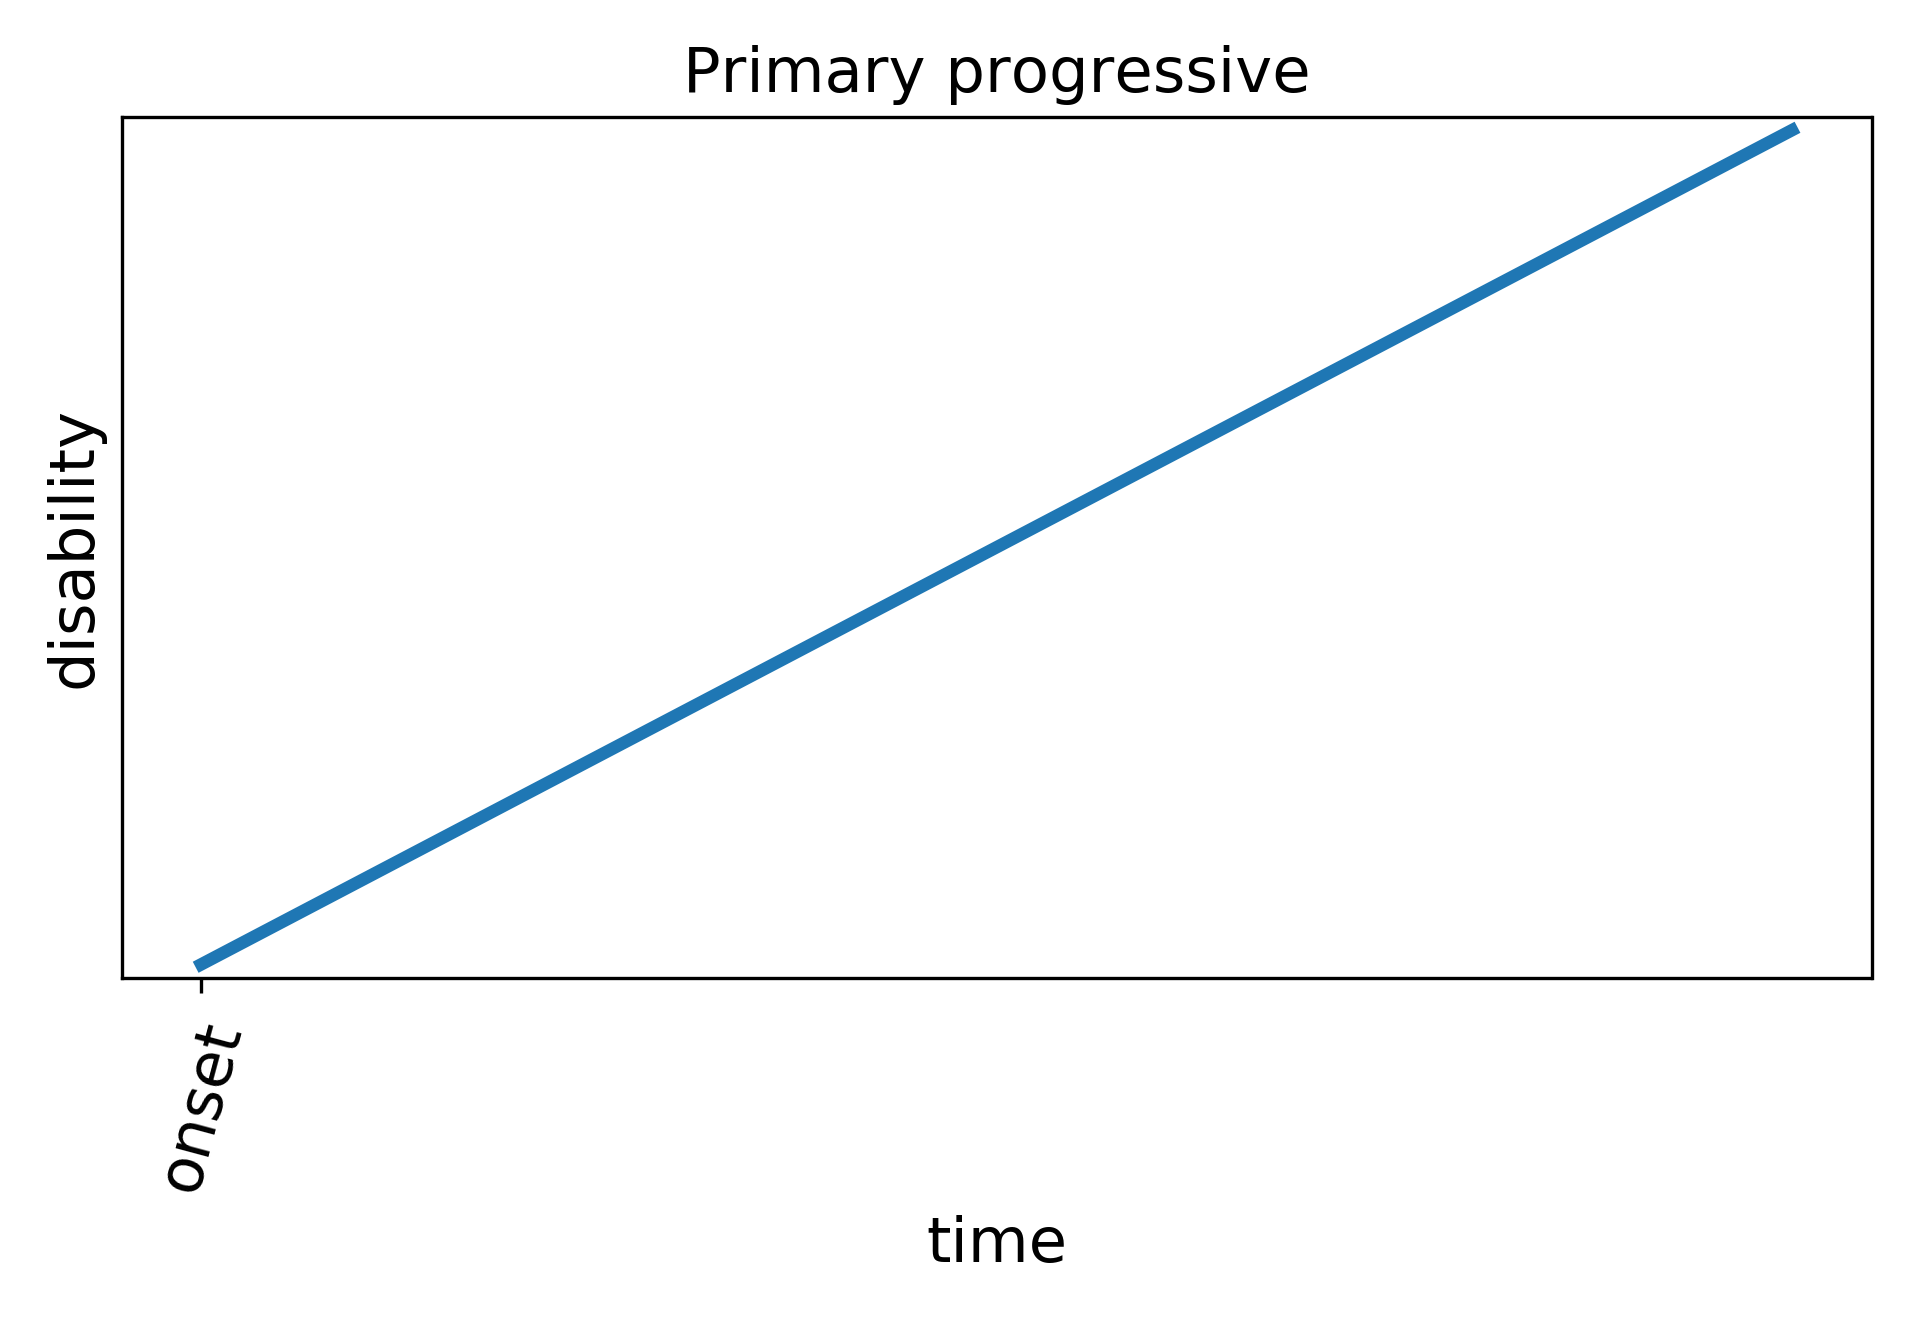
\includegraphics[width=0.5\textwidth]{part2/ms_mock_pp.png}
		\label{fig:ms_mock_pp}%
	}
	\caption{Disability evolution of the four main MS courses: panel (a) shows a prototypical \RR patient, characterized by time-limited attacks which may or may not leave permanent deficits; panel (b) shows \SP typical disability progression, that is steady with no more relapses; panel (c) represents a typical \PR disability evolution, which is characterized by steady disability progression from the onset; panel (d) shows a \PR patient; which has a steady disability progression from the onset with relapses.} \label{fig:ms_mock}
\end{figure}


% This form is characterized by clearly defined {\em relapses}, \ie  attacks of neurological worsening, followed by partial or complete recovery.
% and it takes only $14$ years on average for people to become unable to walk for $100$ meters unaided .
% Patients in \SP form experience a steady progress of the disease in absence of relapses, while patients in \PR form are characterized by both relapses and gradual worsening.

For this reason, the prediction of the transition from \RR to \SP is one of the most important methodological gaps that MS researchers are currently addressing.
The availability of a statistical model able to predict disease worsening is one of the major unmet needs that could significantly improve timeliness, personalization and, consequently, the efficacy of the treatments.
Nowadays, there are no clear clinical, imaging, immunologic or pathologic criteria to foresee the transition from \RR~to~\SP~\cite{lublin2014defining}. Several clinical factors relating to possible \SP course predictors have been identified~\cite{bergamaschi2015bremso, dickens2014type}.
However, as showed by~\cite{vukusic2003prognostic}, studies investigating on prognostic factors for MS course evolution generally suffer from two shortcomings: they
% However, such studies generally
report a high proportion of \RR patients not monitored enough to reach progressive course and they lead, to some extent, to contradictory results.
Currently, MS research mainly focuses on developing and assessing drugs and rehabilitative protocols for \RR patients disregarding progressive courses.

\section{\PCOs data collection}\label{sec:proms_data_collection}

In the recent past, researchers explored the potential role of Patient-Centered Outcomes (\ac{PCO}) to follow the progression of neurodegenerative diseases and to take timely decisions~\cite{black2013patient}. %~\todo{REF \cite{??}}.
%\PCOs usually consist in ordinal or categorical scaled questionnaires and self-reported measures.
\PCOs comprise self- and physician-administered tests, questionnaires and clinical scales consisting of either ordinal or categorical scaled answers.
As opposed to stressful, not frequently repeatable and expensive clinical exams, like magnetic resonance imaging or blood tests, \PCOs are patient-friendly and low-cost measures that could allow to investigate the individual changes and disease impact on several aspects such as physical, cognitive, psychological, social and well-being domains~\cite{fiorini2015machine}.
%.
To date, \PCOs are extensively used to assess general health status, to support diagnosis and monitor progress of disease and to quantify the patients' perception of the effectiveness of a given therapy or procedure \cite{nelson2015patient}.
Nevertheless, it is still unclear which are the most informative \PCOs and, contextually, whether they can be used as {\em predictors} for disease evolution.

%\todo{In our study, we propose a machine learning approach that, leveraging on \PCOs data, aims at
%forecasting the transition of PwMS from \RR to \SP and at providing insights on the most appropriate use of \PCOs.}
%In our study, we propose a machine learning approach that, leveraging on \PCO data, aims at predicting the temporal evolution of MS disease course providing insights on the most appropriate use of \PCOs.
%We resort to a vast category of predictive models, ranging from sparse regularization to ensemble and deep learning methods.
%These models are widely adopted in the biomedical context as they benefit from good generalization properties as well as they allow to address regression and classification problems within the same statistical and computational framework~\cite{lecun2015deep, qi2012random, nowak2011fused,  teramoto2009balanced, zou2005regularization}.
%azencott2013efficient

% \PCOs are low-cost and patient-friendly source of information that can be acquired over time in order to quantitatively assess patients' disease impact on several aspects of their life.

The biomedical data science challenge presented in this chapter is based on a \PCO dataset acquired from a cohort of PwMS progressively enrolled within an ongoing funded project \footnote{ Ethical review committee approval \textit{023REG2014} was obtained for this work.}.

Each patient is evaluated every four months through the items of the \PCOs reported in Table~\ref{tab:proms} which cover physical, cognitive and psychosocial domains. A comprehensive description of the \PCOs involved in the study is presented below.


\begin{itemize}
	\item[] {\sc \textbf{MFIS}} This is a $21$-item self-reported questionnaire typically administered in $5$ to $10$ minutes. \MFIS provides an assessment of the effects of fatigue in terms of physical, cognitive, psychosocial functioning and it is considered a valuable tool by clinicians.
	
	\item[] {\sc \textbf{HADS}} This is a $14$-item self-reported questionnaire typically administered in $2$ to $6$ minutes which aims at detecting clinically significant symptoms of depression and anxiety in patients. \HADS consists in $7$ questions for depression and the remaining $7$ for anxiety.
	
	\item[] {\sc \textbf{LIFE}} This is an $11$-item self-reported questionnaire which investigates on patients quality of life. \LIFE can be typically administered in approximately $5$ minutes. To each of the $11$ items, the patient can assign an ordinal score $0,1,2$ which corresponds to "\textit{disagree}", "\textit{not sure}" and "\textit{agree}" answers.
	
	\item[] {\sc \textbf{OAB}} This is an $8$-item self-reported questionnaire which investigates on patients bladder control. \OAB can be administered in approximately $5$ to $8$ minutes and it is a reliable tool to investigate on possible stress or discomfort lead by unexpected urinary urgencies that patients may experience during day or night.
	
	\item[] {\sc \textbf{EDINB}} This $10$-item self-reported questionnaire can be used to assess dominance of a person's right/left hand during daily activities. The items are very straightforward, so \EDINB can be administered in $3$ to $5$ minutes.
	
	\item[] {\sc \textbf{ABILH}} This is a $23$-item self-reported questionnaire which can be used to measure hand ability in adults with upper limb impairments. \ABILH assesses a person's ability to manage daily activities that require the use of the upper limbs, whatever the strategies involved. \ABILH is usually administered in $5$ to $10$ minutes.
	
	\item[] {\sc \textbf{FIM}} This is $19$-item clinical scale assessing the amount of assistance required for the patient to carry out activities of daily living. \FIM is typically administered by trained examiner in $35$ to $40$ minutes and it covers both motor and cognitive domains.

	\item[] {\sc \textbf{MOCA}} This is an $11$-item clinical scale assessing several cognitive domains such as short-term memory recall, visuospatial abilities, phonemic fluency, attention, concentration and so on. \MOCA is typically administered in less than $10$ minutes.
	
	\item[] {\sc \textbf{PASAT}} This clinical scale is a measure of cognitive function that assesses patients' auditory processing speed and flexibility,  as well as their calculation ability. It can be administered in $10$ to $15$ minutes and it consists in audio stimuli in which single digits are presented every $3$ seconds. The patient is asked to add each new digit to the one immediately prior to it. \PASAT must be administered by trained examiner.
	
	\item[] {\sc \textbf{SDMT}} This clinical scale is a test for organic cerebral dysfunctions. This test simply involves a substitution task: using a reference key the patients has few seconds to pair specific numbers with specific geometric measures.
	\SDMT is typically administered by trained examiner in less than $5$ minutes.
	
	\item[] {\sc \textbf{EDSS}} This is probably the oldest assessment instrument for MS. \EDSS is based on a neurological examination consisting of $7$-items. Each item rates a different function, all the items are then combined in the final \EDSS score which is an ordinal scale ranging from $0$ (normal neurological examination) to $10$ (death due to MS), in half-point increment. The use of \EDSS in modern MS assessment is somewhat controversial. Although usually adopted as an index of the disability level, \EDSS focuses mainly on deambulation disability without taking into account other aspects that could impact patient disability, such as upper limb or cognitive functions~\cite{meyer2014systematic, uitdehaag2014clinical}.
	
	
\end{itemize}

\PCO data are intrinsically noisy due to the subjectivity of self-reported measures provided by the patients that can be influenced by personal feelings and opinions. In order to ameliorate this issue, $4$ questionnaires out of $10$ are administered by medical staff which is trained to keep a homogeneous level of evaluation.

In our analysis we considered all the \PCOs reported in Table~\ref{tab:proms} except \EDSS.
%\todo{other comments here?}

% The model considered all the \PCOs except \EDSS, that is a physician reported outcome that, although usually adopted as an index of the disability level, exclusively depends on the deambulation for scores greater than 4, consequently not taking into account the other aspects impairing the patient.

\begin{table}[htb]
	\center
	\footnotesize
	\begin{tabular}{l|l|l}%{@{} l*{4}{l} @{}}
		\toprule
		Acronym & Full name & Reference \\
		\midrule
		\MFIS & Modified fatigue impact scale & \cite{flachenecker2002fatigue}\\
		\HADS & Hospital anxiety and depression scale &  \cite{honarmand2009validation}\\
		\LIFE &  Life satisfaction index &  \cite{franchignoni1999life}\\
		\OAB & Overactive bladder questionnaire & \cite{cardozo2014validation}\\
		\EDINB &  Edinburgh handedness inventory & \cite{oldfield1971assessment} \\
		\ABILH &  Hand ability index & \cite{arnould2012can} \\
		\midrule
		\FIM &  Functional independence measure  &\cite{granger1990functional}\\
		\MOCA &  Montreal cognitive assessment & \cite{dagenais2013value}\\
		\PASAT &  Paced auditory serial addition task & \cite{aupperle2002three} \\
		\SDMT &  Symbol digit modality test  & \cite{parmenter2007screening}\\
		\EDSS & Expanded disability status scale & \cite{kurtzke1983rating}\\		\bottomrule
	\end{tabular}
	\caption{The set of available \PCOs.
		The first $6$ are self-reported, while the last $5$ are administered by trained medical staff.
		In our analysis all \PCOs were used, with the exception of \EDSS.
		% The set of clinically validated questionnaires available for this work. All questionnaires were used to predict the disease course evolution with exception of \EDSS. The answers to the first $6$ questionnaires are completely self-reported, while the last $5$ are administered by trained medical staff.
	}\label{tab:proms}
\end{table}


% we focus on the use of $10$ of the clinically validated questionnaires reported in Table~\ref{tab:proms}. Each questionnaire consists of a different number of items testing the capabilities of the patients in different domains, such as physical, cognitive or psychosocial.
% Moreover, the set of variables considered by our
The collected \PCO dataset comprises additional information such as:
\begin{enumerate*}[label=\roman*)]
	\item number of relapses in the last four months (NR),
	\item educational level expressed in terms of total years of education (EDU),
	\item height (H) expressed in $\text{cm}$ and
	\item weight (W) expressed in $\text{kg}$.
\end{enumerate*}
Moreover, a neurologist assigns to each patient the corresponding disease course. The global distribution of MS types across time points is depicted in Figure~\ref{fig:PPRRSP}.

% \todo{@AISM: add here the motivations that lead us to exclude \EDSS from the analysis.}

%%%%%%%% EDA %%%%%%%%
\section{\PCOs exploratory data analysis} \label{sec:aism_eda}

%In this work we focus on detecting the \RR to \SP prediction, hence the patients in \PR and \PP form will not be taken into account.

In this work we analyze \PCOs data acquired every four months from a cohort of MS patients enrolled in a funded study.
Currently, we have collected data for $11$ examinations and, as patients enrollment is still ongoing,  the number of individuals for each time point is successively decreasing, as shown in Figure~\ref{fig:patients}.
\begin{figure}[]
	\centering
	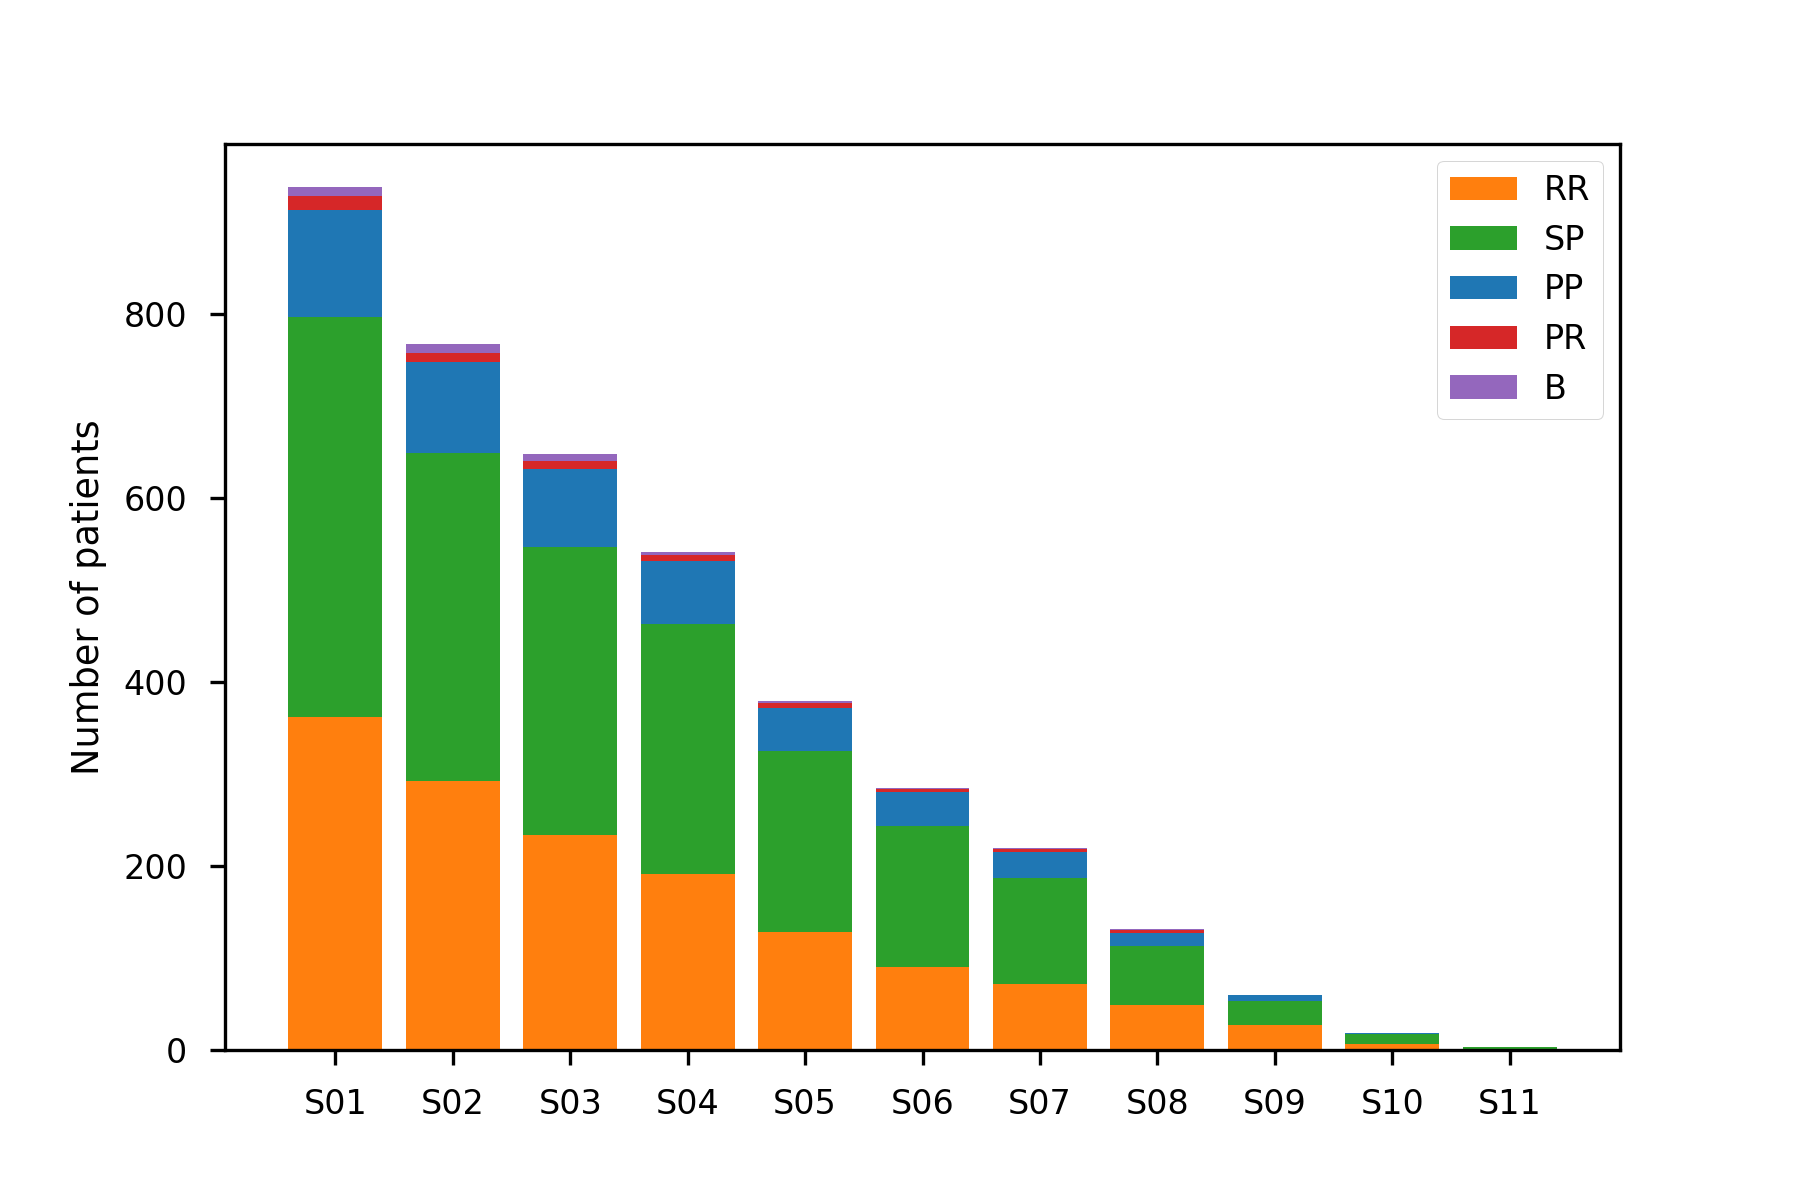
\includegraphics[width=0.8\textwidth]{part2/ms_bars.png}
	\caption{Bar chart of the number of MS patients in each disease form  at different examinations.} \label{fig:patients}
\end{figure}

The collected dataset comprises a grand total of $3991$ patients, with $1451$ \RR, $1947$ \SP, $503$ \PP, $53$ \PR and $37$ benign cases, as shown in Figure~\ref{fig:PPRRSP}.
\begin{figure}[]
	\centering
	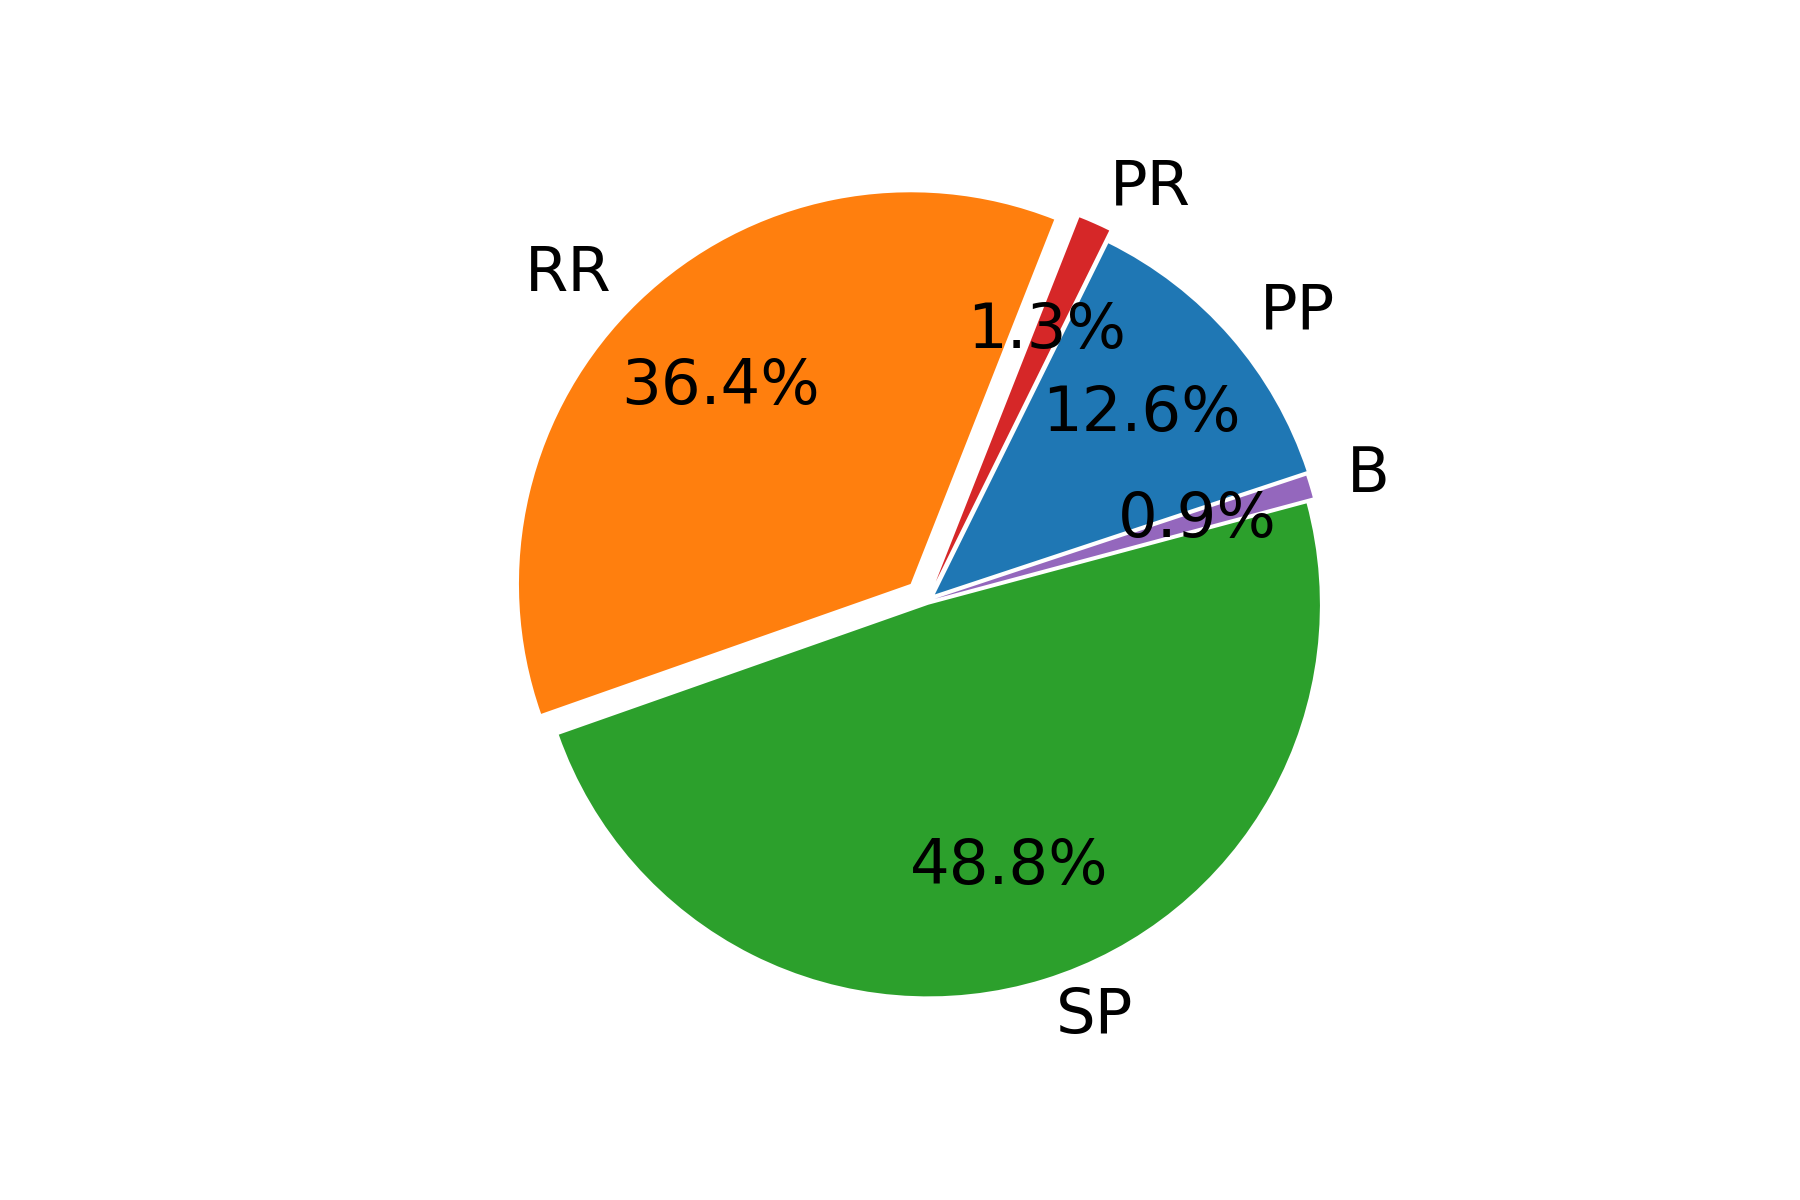
\includegraphics[width=0.8\textwidth]{part2/ms_pie.png}
	\caption{Representation of the distribution of the total amount of acquisitions, divided according to the disease form.} \label{fig:PPRRSP}
\end{figure}

Each sample of the dataset is represented by a vector containing the $145$ predictors summarized in Table~\ref{tab:proms}.
As the missing data ratio amounts to $1.61\%$ of the entire dataset, we resort to the $k$-nearest neighbor data imputing strategy (with $k=3$) proposed in~\cite{troyanskaya2001missing}.

Analyzing \PCO data is challenging from several respects.
For instance, items belonging to different questionnaires are encoded with numerical values in different ranges.
For example, the items of the \MFIS questionnaire have ordinal scale values in $[0-4]$, whereas the \SDMT outcome is the global number of correctly answered items of the test (max $110$) and the \EDINB test consists in $10$ categorical items measuring the dominance of right or left hand in the activities of daily living.
To tackle such issues, in this EDA we opted for a preliminary data preprocessing of the ordinal answers and a binary one-hot-encoding of the categorical ones, the latter increases the dimensionality of the samples, leading to $d=165$ variables in the dataset.
The adopted data preprocessing strategy, namely min-max scaling, consists in casting each feature $x^j$ in a fixed range, \ie $x^{j'} \in [0, 1]$. The min-max scaling is obtained by the transformation described in Equation~\eqref{eq:minmax}.
\begin{equation} \label{eq:minmax}
	x^{j'} = \frac{x^j - \min(x^j)}{\max(x^j) - \min(x^j)}
%	X_std = (X - X.min(axis=0)) / (X.max(axis=0) - X.min(axis=0))
\end{equation}
The effect of the data preprocessing on the ordinal input variables is visually represented in Figure~\ref{fig:ms_boxplots}. As we can see, this preprocessing step allows to compare more easily the input features.

\begin{figure}[]
	\centering
	\subfloat[]{%
		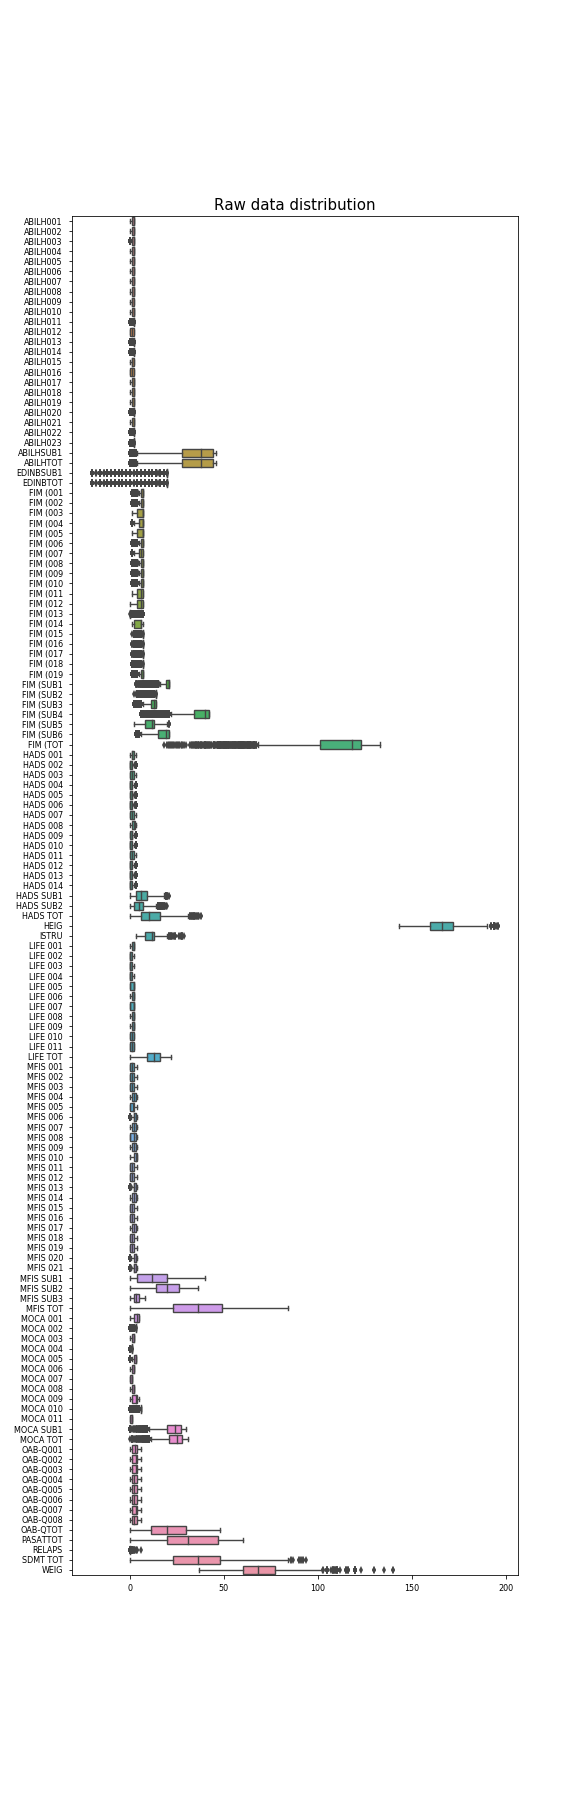
\includegraphics[trim={0 6cm 0 6cm}, width=0.5\textwidth]{part2/ms_raw_boxplot.png}
		\label{fig:ms_boxplots_pre}%
	}%
	%	\hfill%
	\subfloat[]{%
		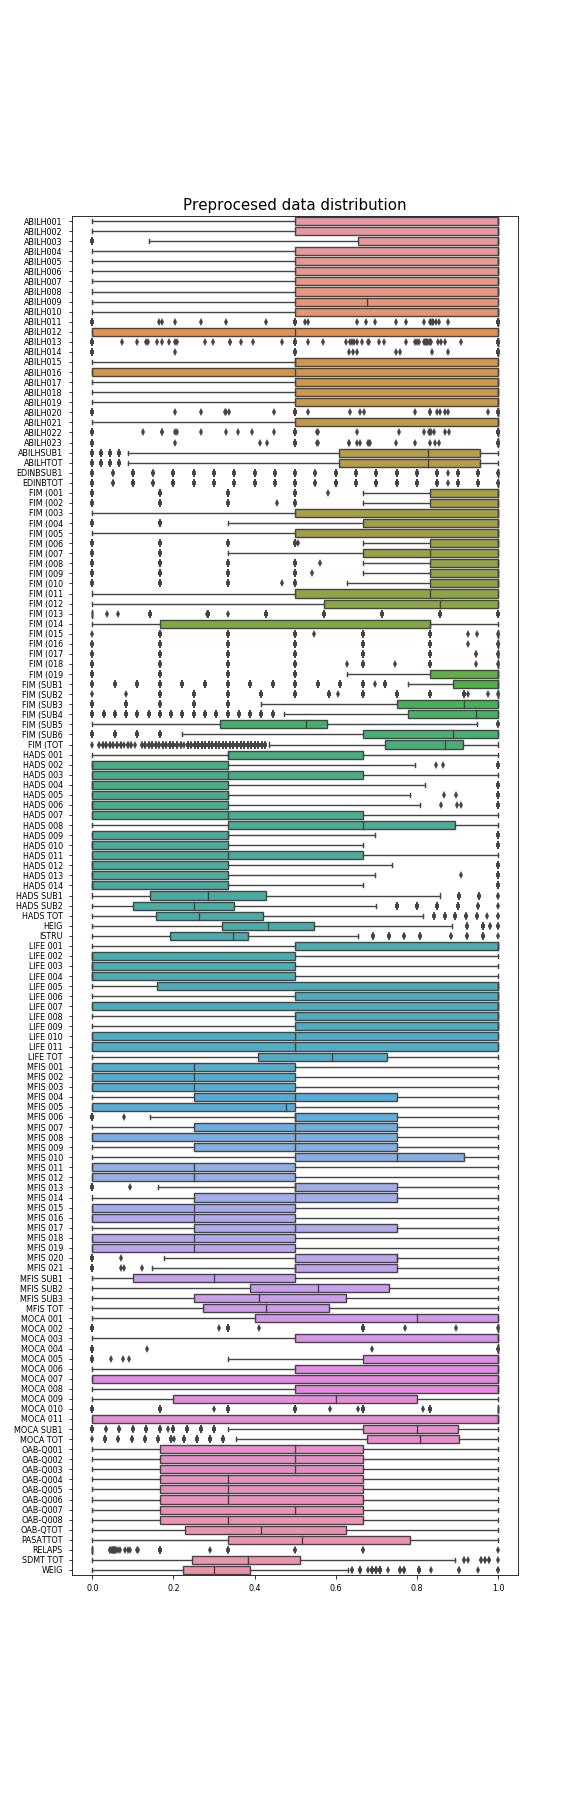
\includegraphics[trim={0 6cm 0 6cm}, width=0.5\textwidth]{part2/ms_mm_boxplot.png} \label{fig:ms_boxplots_post}
	}%
	\caption{The effect of the data preprocessing on the input ordinal \PCOs. The left panel (a) shows the distribution of the raw collected variables, whereas the right panel (b) shows the distribution of the same variables after the preprocessing step.}\label{fig:ms_boxplots}
\end{figure}

Furthermore, in order to visually inspect the data we investigate on how to reduce their dimensionality. To this aim, we project the data in a 3D space with linear PCA and Isomap (see Section~\ref{sec:dimred}).
These algorithms are sensitive to outliers, which we expect to affect our dataset. Therefore, we follow a preliminary isolation forests-based anomalies detection and removal as described in~\cite{liu2008isolation, liu2012isolation}.
The obtained scatter plots are shown in Figure~\ref{fig:ms_3dscatterplot}.
As we can see, both the obtained projections hint some sort of class separation between \RR and \SP subjects, while the same conclusion cannot be drawn for the other classes. Moreover, considering only the first three principal components, PCA explains only the $37.4\%$ of the variance of the dataset. This suggests that most of the information, which may be useful for classification purposes, is spread across several input variables.
%in this dataset the low dimensionality projection and visualization is not insightful. From the scatter plots in Figure~\ref{fig:ms_3dscatterplot} a clear class separation cannot be firmly observed.

\begin{figure}[h!]
	\centering
	\subfloat[]{%
		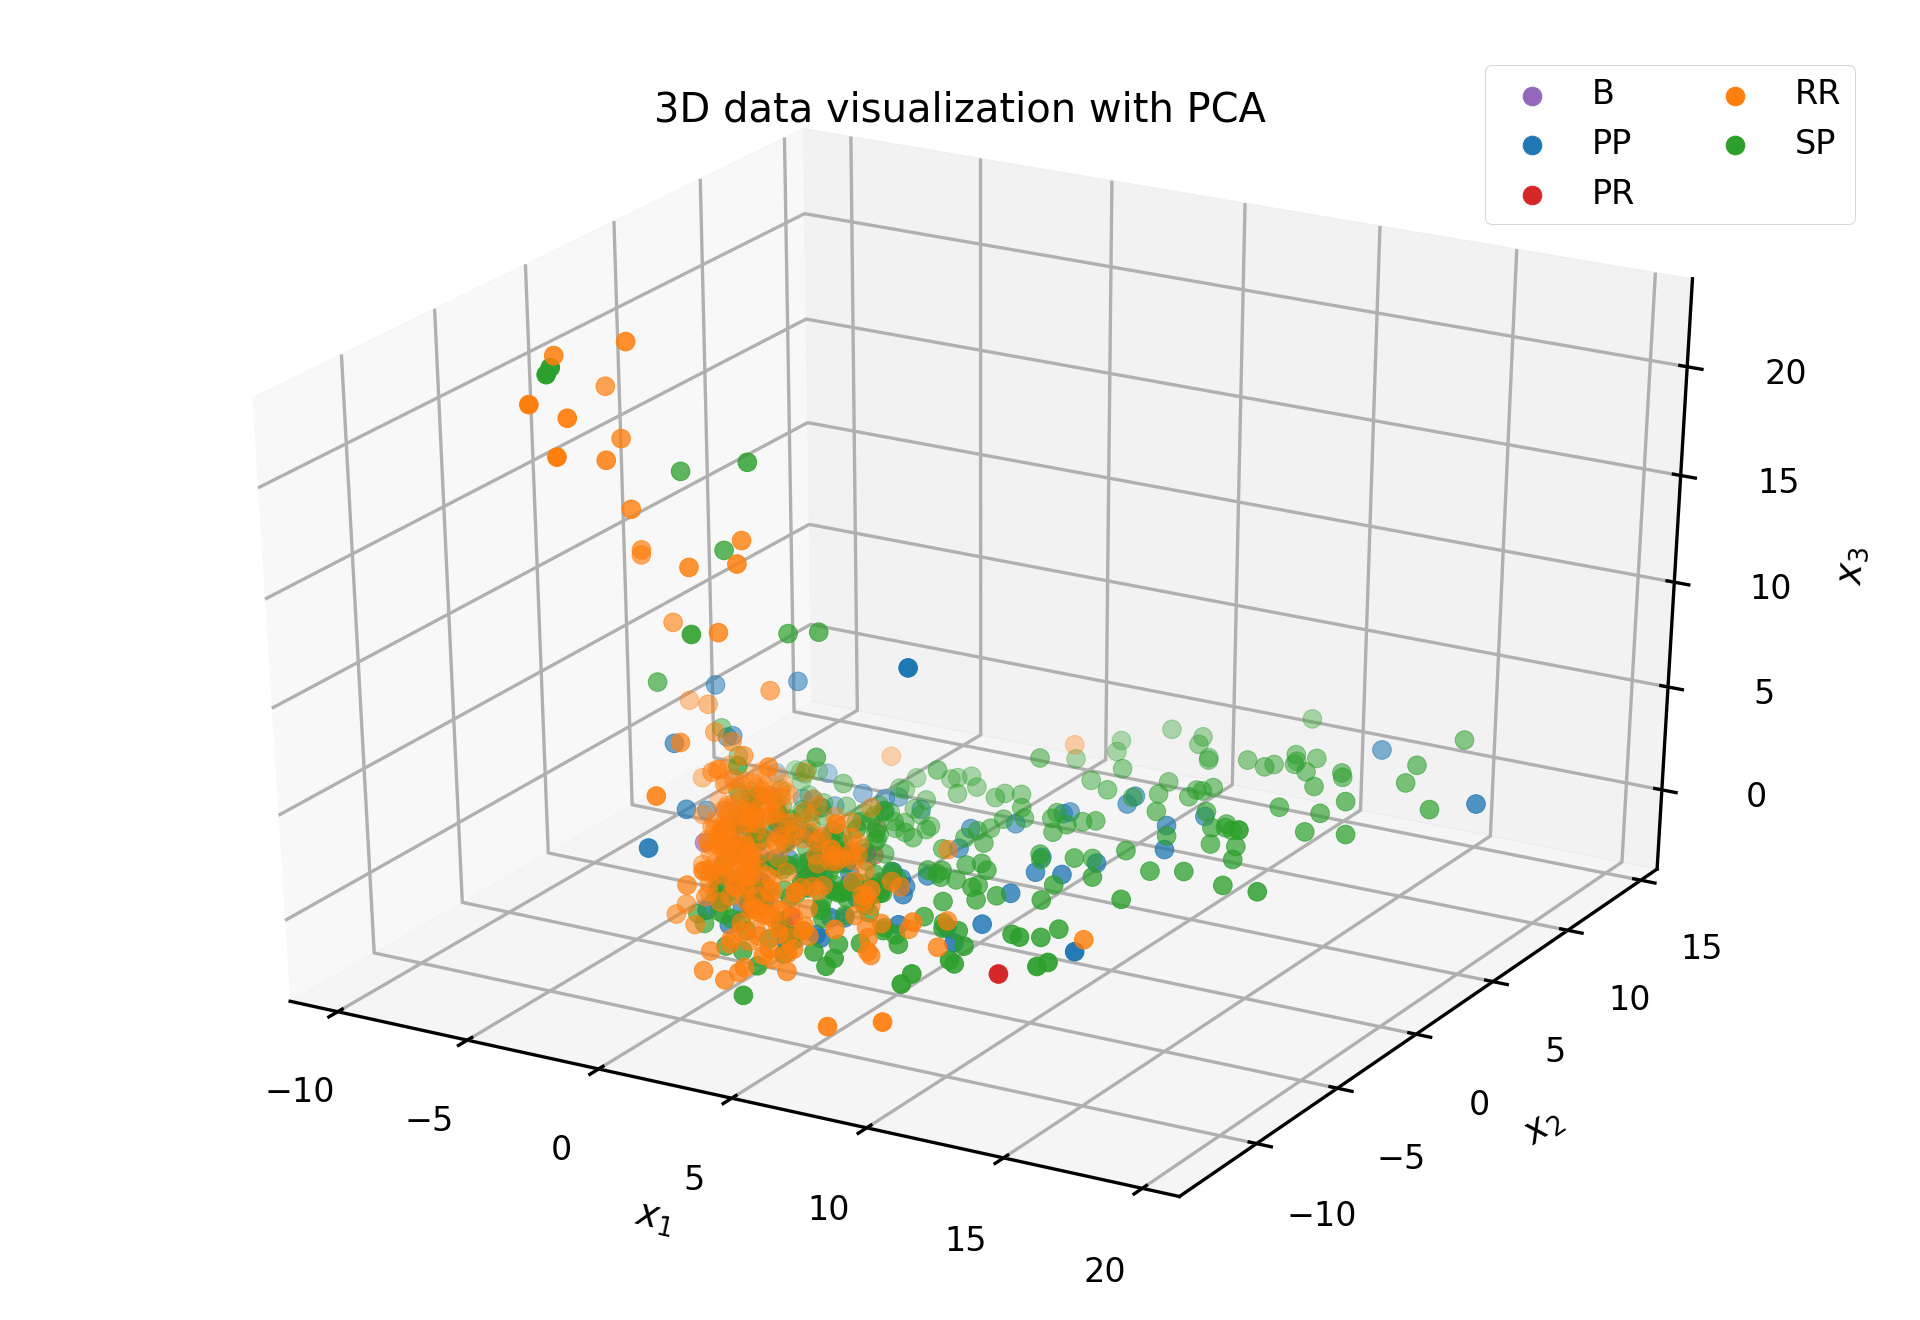
\includegraphics[width=0.5\textwidth]{part2/ms_pca.png}
		\label{fig:ms_ms_pca}%
	}%
%	\hfill
	\subfloat[]{%
		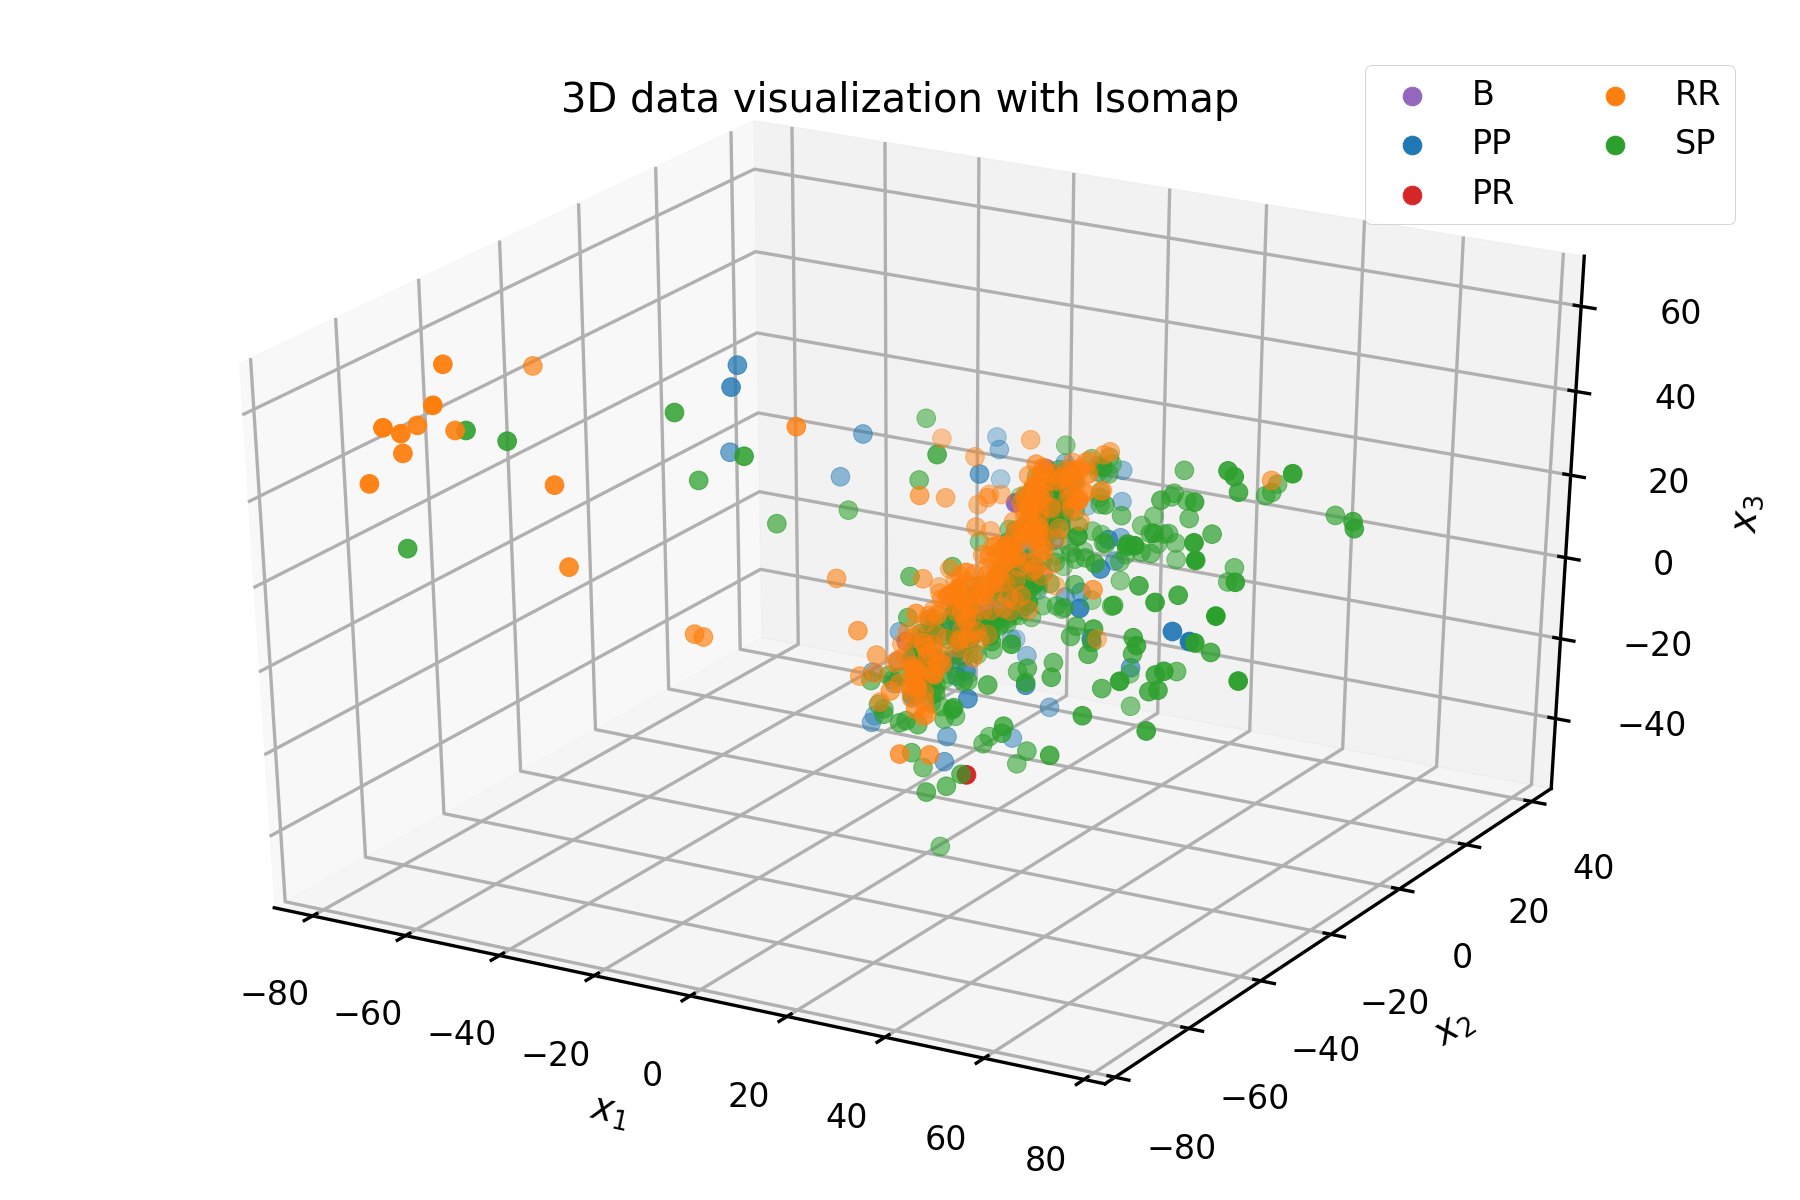
\includegraphics[width=0.5\textwidth]{part2/ms_isomap.png}
		\label{fig:ms_ms_isomap}%
	}
%	\subfloat[]{%
%		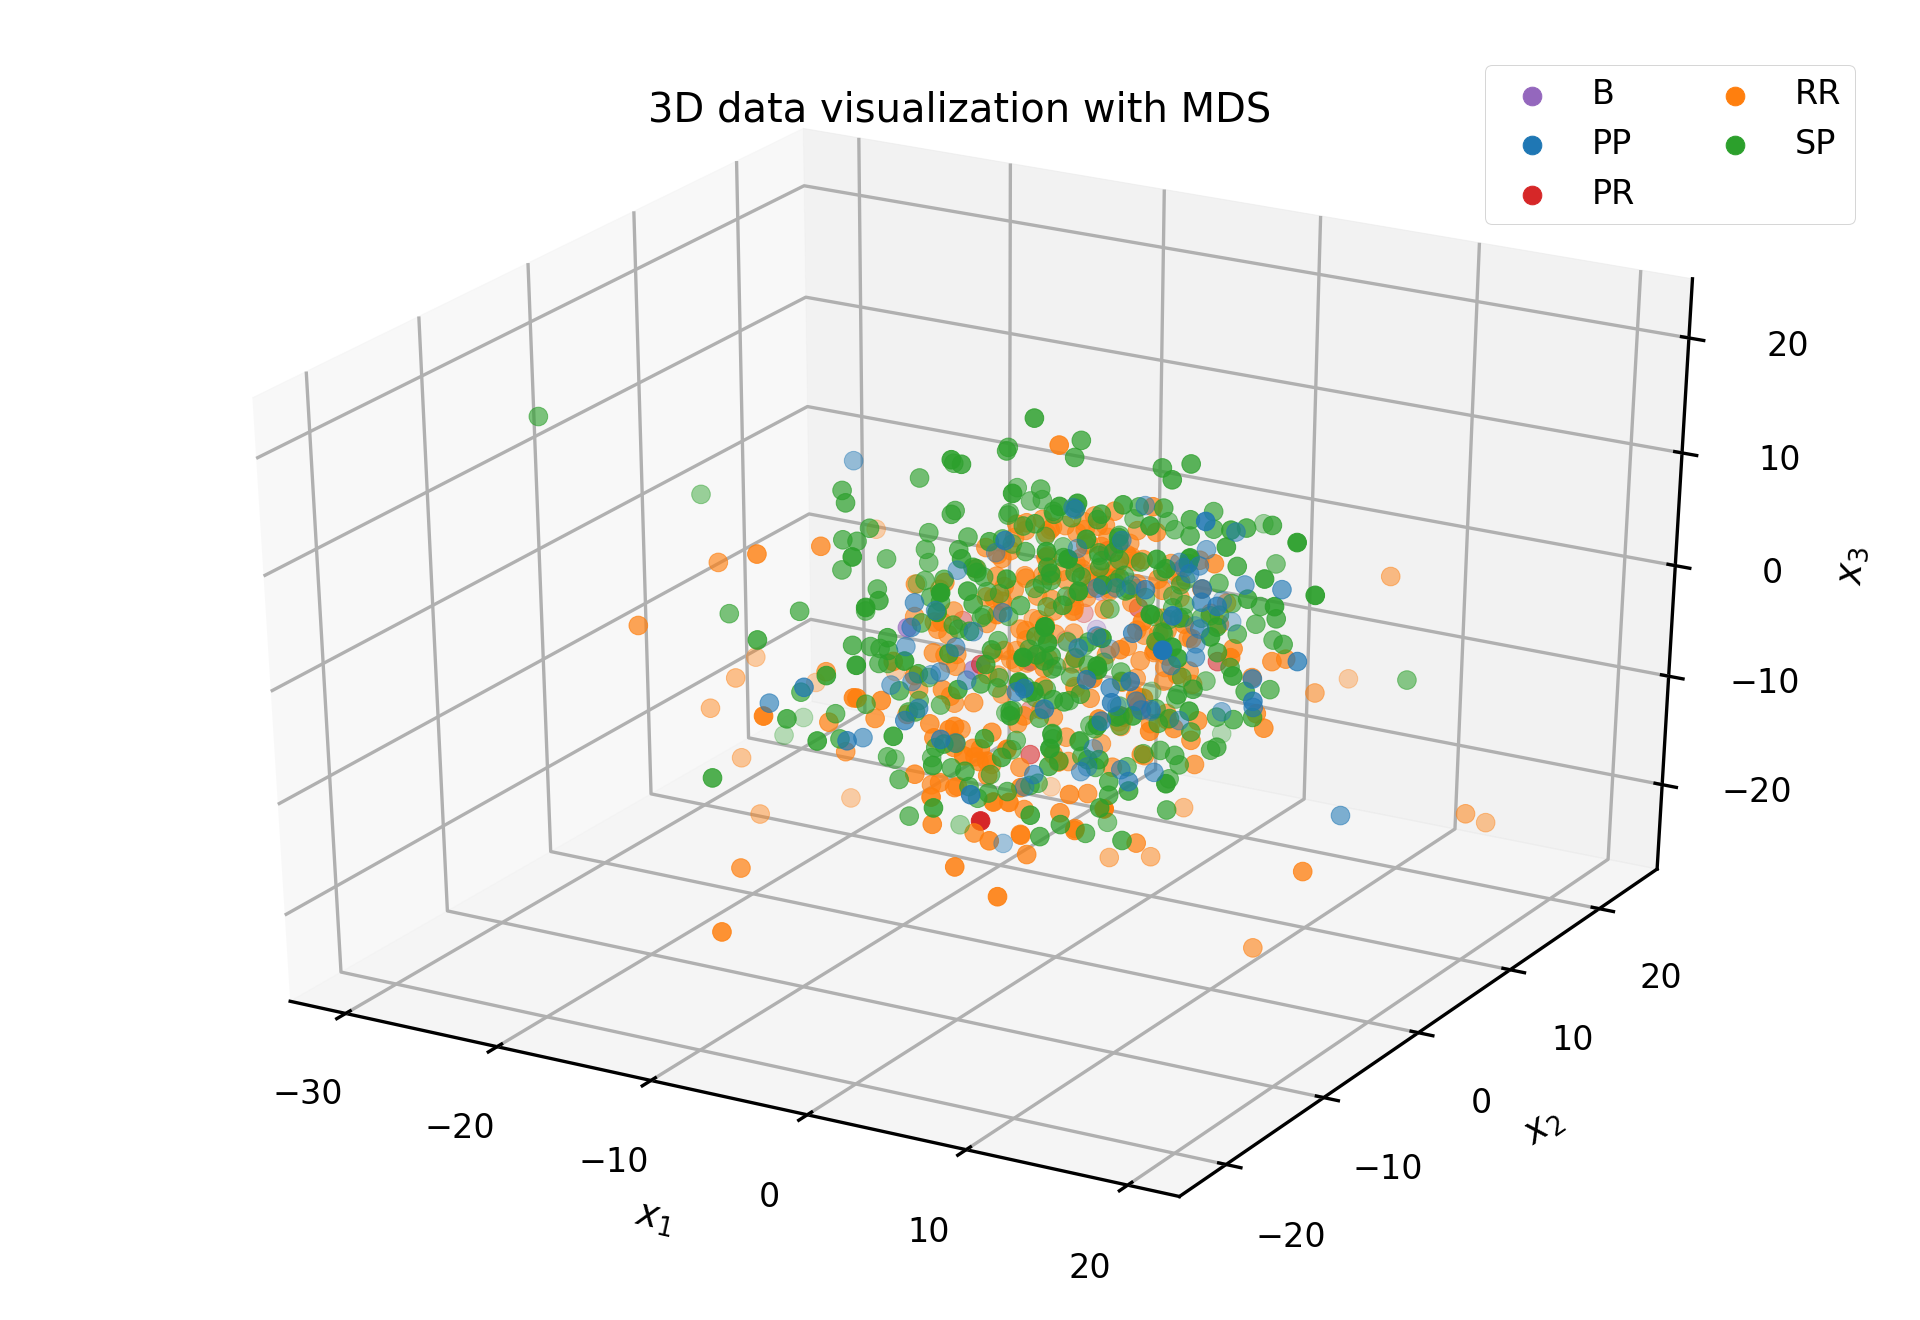
\includegraphics[width=0.5\textwidth]{part2/ms_mds.png}
%		\label{fig:ms_ms_mds}%
%	}%
%	\subfloat[]{%
%		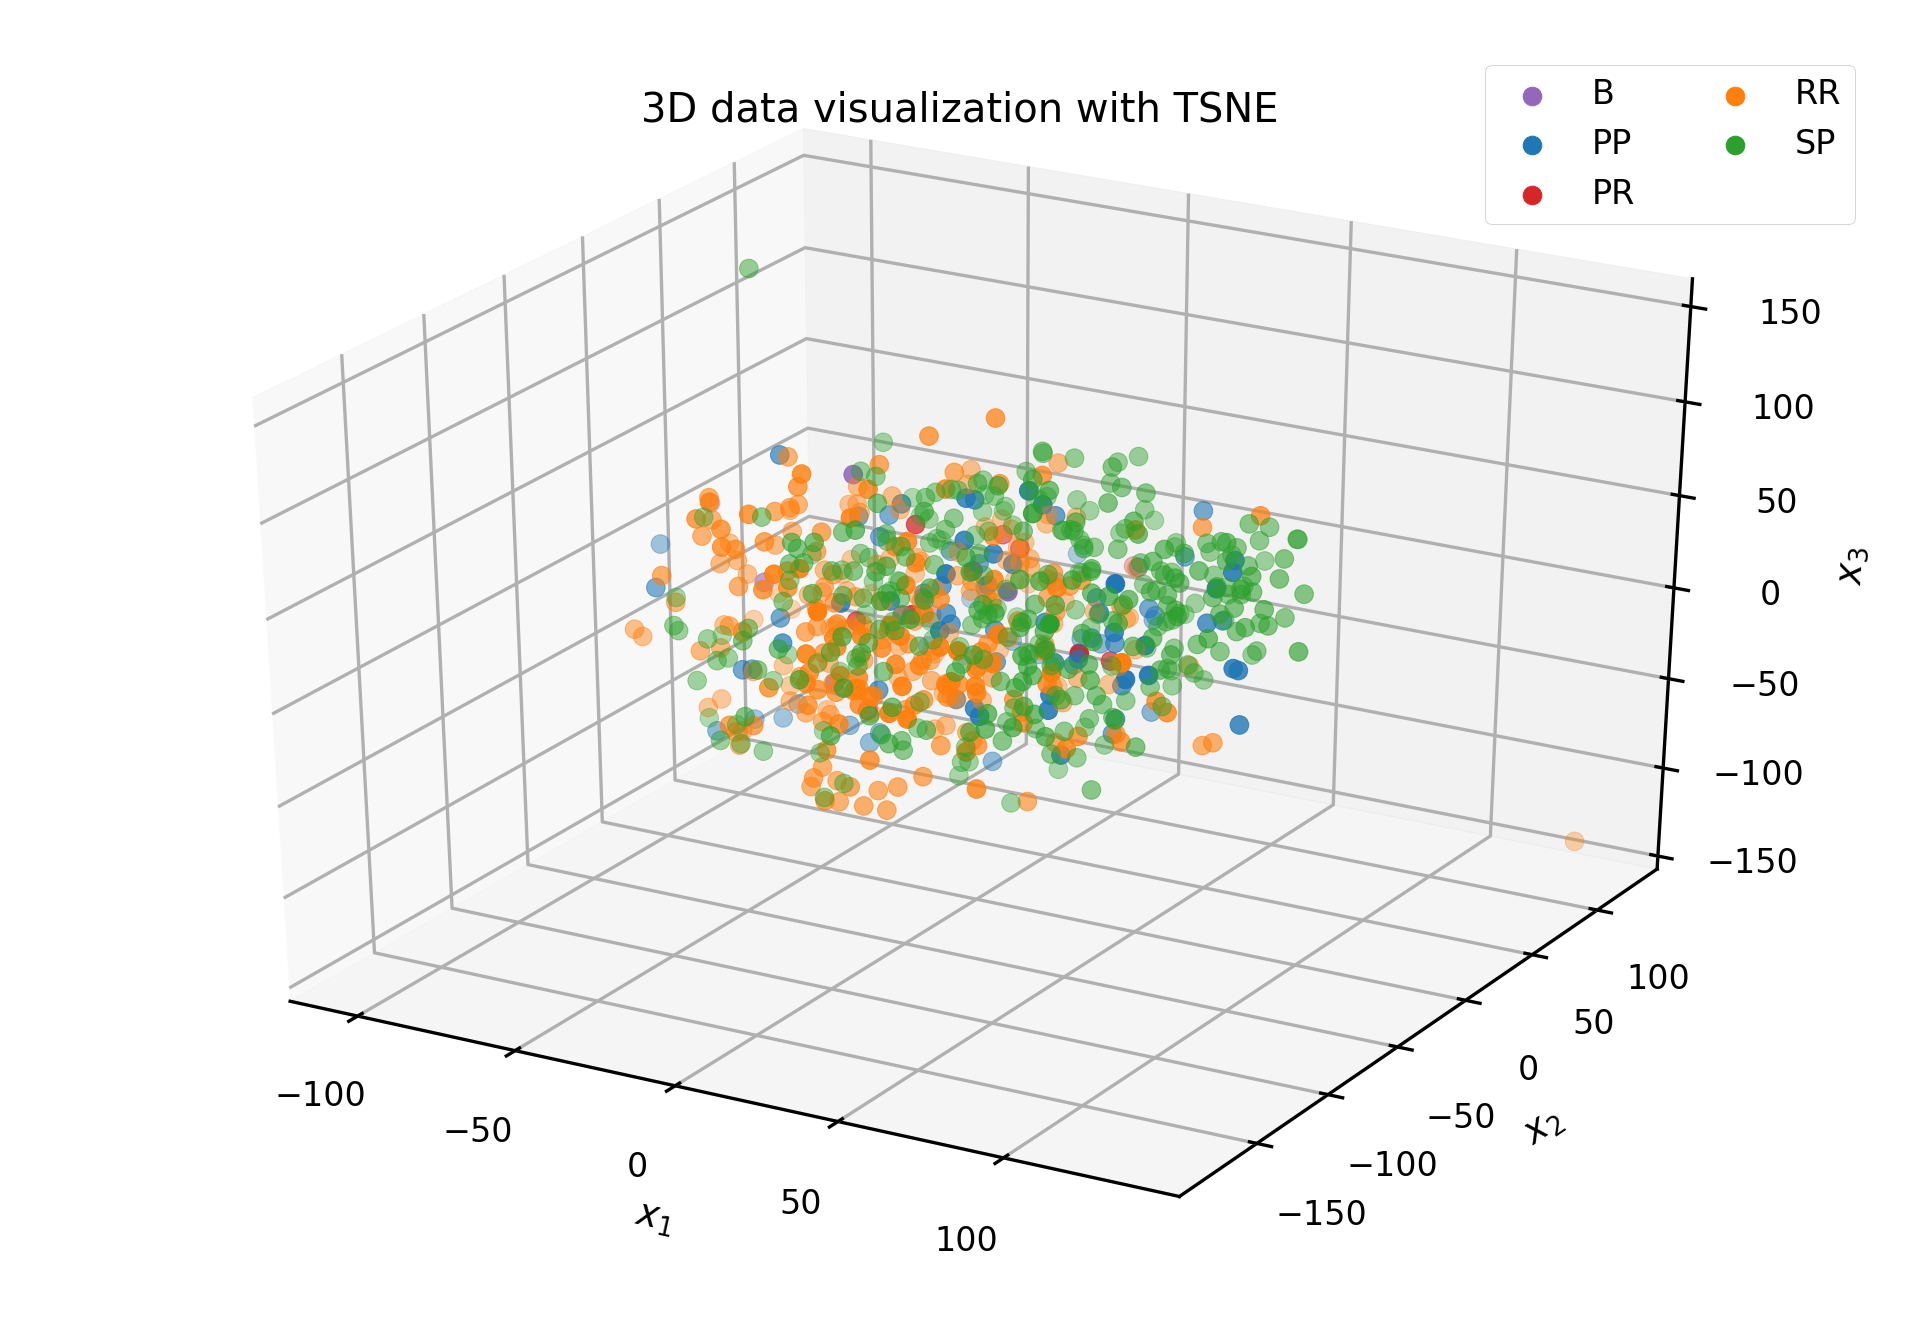
\includegraphics[width=0.5\textwidth]{part2/ms_tsne.png}
%		\label{fig:ms_ms_tsne}%
%	}
	\caption{A random extraction of the $20\%$ of the MS dataset projected on a 3D space by linear PCA, on panel (a), and Isomap, on panel (b).} \label{fig:ms_3dscatterplot}
\end{figure}

This EDA raised our hopes to successfully perform a further supervised MS course classification and evolution prediction.

% The number of considered samples across examinations is hence $2699$, of which $1220$ \RR and $1579$ \SP.


\section{Supervised analysis}\label{sec:problem_description}

% We adopted suitable categorical data encoding and missing values imputing strategies to cope with these issues (see Section~\ref{sec:problem_description}).

%a machine-learning based temporal model that, extracting information from \PCOs data, is able to answer to
In order to develop a temporal model of MS evolution, we assume that our data can be modeled according to the temporal structure outlined in Figure~\ref{fig:pipeline}.
Therefore, predicting the MS course evolution can be split in three different related tasks, which we call: \f (\F), \g (\G) and \fog (\FOG).


% documentclass[letter,10pt]{article}
% \usepackage{amsmath}
% \begin{document}

\begin{figure}[]
  \centering
  \begin{tikzpicture}[->, >=stealth', auto, semithick, node distance=4cm]
    \tikzstyle{every state}=[fill=white,draw=black,thick,text=black,scale=1, minimum height=2.5cm]
    \node[state]    (xit)                     {$\bm{x}_i^t$};
    \node[state]    (yit)[below of=xit]       {$y_i^t$};
    \node[state]    (xit1)[right of=xit]      {$\bm{x}_i^{t+1}$};
    \node[state]    (yit1)[below of=xit1]     {$y_i^{t+1}$};
    \path
    (xit)  edge node{$f$} (yit)
    (xit)  edge node{$g$} (xit1)
    (xit1) edge node{$f$} (yit1)
    (xit)  edge node{$f\circ g$} (yit1);
  \end{tikzpicture}
  \caption{A visual representation of the temporal structure assumed in the collected data. When the two functions $f$ (\F) and $g$ (\G) are learned, the \FOG model $f\circ g$ is able to predict the evolution of the disease course for future time points $y_i^{t+1}$.}\label{fig:pipeline}
\end{figure}
% \end{document}



\begin{enumerate}
	\item[] \textbf{\F} Given the $165$-dimensional representation of a patient at a fixed time point $\bm{x}_i^t$, this task consists in assigning the corresponding disease course $y_i^t$. \F can be translated into a binary classification problem which can be solved by learning a discriminative function $f(\bm{x}_i^{t}) = y_i^{t}$.
	
	\item[] \textbf{\G} Given the historical representation  of a patient $\bm{x}_i^t$ for $t=1,\dots,\tau$, this task consists in predicting the patient representation $\bm{x}_i^{\tau+1}$. \G can be seen as a multiple-output regression function and it can be solved by learning an appropriate function $g(\bm{x}_i^{t}) = \bm{x}_i^{t+1}$.
	
	\item[] \textbf{\FOG} This task can be seen as foreseeing the MS disease course $y_i^{\tau+1}$ from $\bm{x}_i^t$ for $t=1,\dots,\tau$. Once $\hat{f}(\bm{x})$ and $\hat{g}(\bm{x})$ are learned by training on historical \PCO data, the \FOG problem is finally solved by the temporal model $\hat{f} \circ \hat{g}(\bm{x}_i^{t}) = y_i^{t+1}$. In time-series data analysis, this is known as \textit{one-step-ahead forecast}. Notably, the \FOG model allows to foresee if the patient at the next time point is likely to experience a transition from \RR to \SP, or not.

\end{enumerate}


\subsection{Experimental design}\label{sec:experimental_design}
Our final goal is predicting MS course evolution of  \RR and  \SP patients, hence the subjects with \PR, \PP and benign forms are not further taken into account.

We considered all the patients with a minimum of $1$ time point (the most recently enrolled) up to $T=11$ time points for a total of $3398$ samples, of which $1451$ \RR and $1947$ \SP.
%As this is an ongoing project, the number of PwMS decreases with time.
%We expect to fill the gap of samples between \textit{Exam~$1$} and \textit{Exam~$11$} by the end of the funded study.
Following the EDA, we opted for a preliminary feature-wise min-max scaling.
However, to promote unbiasedness of the results, this preprocessing phase is not performed on the entire data collection, but it is embedded into the model fitting procedure. This trick, jointly applied with cross-validation techniques, guarantees that even the feature-wise range used for data preprocessing is \textit{learned} from training set and it is applied on previously unseen validation sets.
%separately evaluated prior to each model fitting process on its training cross-validation portion of the data.
However, the experimental design adopted to learn $f(\bm{x})$ and $g(\bm{x})$ is slightly different. Therefore, each of them is separately discussed in the remainder of this section.

% In particular, the training set comprises all samples collected at time points $t = 1, \dots ,T_{tr}$, the validation set at $t=T_{tr}+1,\dots,T_{vld}$ and the test set at $t=T_{vld}+1,\dots,T$.
% Here, as the maximum number of collected time points is $T=8$, we fixed $T_{tr} = 3$ and $T_{vld} = 4$.
% In particular, the training set comprises all samples collected at time points $t = 1, \dots ,T_{tr}$, the validation set at $t=T_{tr}+1,\dots,T_{vld}$ and the test set at $t=T_{vld}+1,\dots,T$.

\begin{itemize}
	\item[] \textbf{\F} The \F model $f(\bm{x})$ solves a binary classification problem: to each input $\bm{x}_i^t$ is associated  an output $y_i^t$ that encodes the corresponding MS disease course (\RR or \SP) with a binary label.
	We split the dataset in three temporal chunks, namely \textit{training}, \textit{validation} and \textit{test} sets, consisting of all samples collected at time points $t=1,2,3$, $t=4$ and $t=5,6,7,8,9,10,11$, respectively.
	Accordingly, we used $1993$ samples for training $f(\bm{x})$, $463$ for validation leaving the remaining $942$ for test.
	
	Seven candidate models, see Section~\ref{sec:learning_f}, for $f(\bm{x})$ are fitted on $100$ Monte Carlo random sampling of the training set each time keeping $\frac{1}{4}$ of the samples aside, see Section~\ref{sec:model_evaluation}. For each Monte Carlo sampling the fitting procedure is performed on the remaining $\frac{3}{4}$ of the samples and it includes an inner parameter optimization via grid-search cross-validation, as described in Section~\ref{sec:model_selection}. In particular, we require the MS course prediction to be based on a reduced number of variables, therefore we enforce sparsity in each candidate model.
	% Each candidate model is required to be sparse, therefore the MS course prediction is based on a reduced number of variables (see Section~\ref{sec:learning_f}).
	Leveraging on this Monte Carlo-based stability selection strategy, we rank the variables according to their selection frequency, see Section~\ref{subsec:feature_selection}.
	Once a variable ranking is achieved for each candidate model, the list of selected variables is identified by thresholding the corresponding ranking with the threshold that maximizes the MCC on the validation set. Finally, the last training step consists in fitting each candidate model on the union of training and validation sets taking only into account the corresponding reduced subset of selected variables. The final \F model $\hat{f}(\bm{x})$ is chosen as the one that performs better on the previously unseen test set in terms of accuracy, MCC, precision, recall and $\text{F}_1$ score.
	These performance metrics for classification are defined in Section~\ref{sec:performance_metrics}.

	\item[] \textbf{\G} %presents the answers provided by the MS patients to the \PCOs questionnaires, while the label vector $\bm{y}$ has the corresponding disease form diagnosis.
	On the other hand, learning the \G model $g(\bm{x})$ implies solving a multiple-output regression problem as to each input $\bm{x}_i^t$ is associated the output vector $\bm{x}_i^{t+1}$.
	% and the class labels are not taken into account.
	Therefore, we can only consider samples at time point $t$ with an available follow-up at the next time point $t+1$, which reduces the overall number of available samples.
	The dataset splitting is consistent with the one followed for learning $f(\bm{x})$, although in this case there is no need for a separate validation set, as learning $g(\bm{x})$ does not require any variable selection process. We used the samples collected at time points $t=1,2,3,4$ for training and those at $t=5,6,7,8,9,10,11$ for test, resulting in $1946$ and $714$ samples, respectively.
	The fitting procedure includes an inner parameter optimization via grid-search cross-validation. Each candidate model is a function
	$g: \mathbb{R}^{165} \rightarrow \mathbb{R}^k$ where $k$ is the number of variables selected by the best \F model.
	% that predicts the evolution of the variables selected by the best \F model starting from the full set of \PCOs.
	Three candidate models are evaluated to solve this problem.
	The final \G model $\hat{g}(\bm{x})$ is chosen as the candidate model that performs better on the previously unseen test set in terms of MAE, defined in Section~\ref{sec:performance_metrics}.
	

	\item[] \textbf{\FOG} The predictive capability of the \FOG model $\hat{f} \circ \hat{g}(\bm{x})$ is finally evaluated on the test set. The \F model $\hat{f}(\bm{x}_i^t)$ predicts the MS course $\hat{y}_i^t$ from the \PCO data vector $\hat{\bm{x}}_i^t$ that, in turn, is predicted by the \G model $\hat{g}(\bm{x}_i^{t-1})$. We shall notice here that the predictions $\hat{f} \circ \hat{g}(\bm{x}_i^t)=y_i^{t+1}$ for $t=11$ are foreseeing possible \RR to \SP transitions that are beyond our data observation, hence predictions at the last time point cannot be used to assess the \FOG model performance. Therefore, its performance is evaluated only on $616$ test samples.
	
\end{itemize}




%Finally, the predictive capability of the prognosis model $\hat{f} \circ \hat{g}(\bm{x})$ is evaluated by predicting $\hat{g}(X_{T-1})=\hat{X}_T$, that is the evolution of the \PCOs for the patients at time point $T-1$, then applying the diagnosis model on the predicted data matrix $\hat{f}(\hat{X}_T)=\hat{y}_T$ and comparing them with the diagnosis provided by the doctors at the same examination.



\subsection{Learning $f(x)$} \label{sec:learning_f}


%First, we will require the diagnosis function $f(\bm{x})$ to be sparse, hence the MS outcome prediction will be based on a reduced number of variables.
We imposed $f(\bm{x})$ to be sparse. This requirement is helpful from two distinct respects:
\begin{enumerate*}[label=(\roman*)]
	\item predictive model performance increases thanks to a reduced effect of the course of dimensionality~\cite{hastie2015statistical} and
	% \item the effect the course of dimensionality~\cite{hastie2015statistical} may be attenuated, hence increasing the performance of the predictive model, and
	\item the identification of a reduced subset of meaningful \PCOs provides easily interpretable results for the clinicians.
\end{enumerate*}

In order to achieve a sparse model, we take advantage of two variable selection strategies: embedded and wrapper methods, see Section~\ref{subsec:feature_selection}.
When using embedded methods, we exploited the sparsity inducing penalties of three models:
\begin{itemize}
	\item the Elastic-Net, that presents square loss and a penalty which is a convex combination of $\ell_1$- and $\ell_2$-norm of the variable weights (see Section~\ref{sec:elastic_net}),

	\item sparse logistic regression, which combines the logistic loss with a Lasso penalty on the variable weights (see Section~\ref{sec:logistic_regression}),
	
	\item $\ell_1$-penalized SVM (see Section~\ref{sec:svm}).
\end{itemize}
We expect Elastic-Net to exploit correlations between \PCOs, which we assume in our dataset. On the other hand, the use of sparse logistic regression and $\ell_1$-penalized SVM can benefit from the renowned classification capability of their loss function.
Moreover, we applied the RFE wrapper method to four other methods:
\begin{itemize}
	\item logistic regression, that achieves smooth solutions thanks to its $\ell_2$-norm penalty;
	\item SVM, which also has an $\ell_2$-norm penalty;
	\item Random Forests (RF), a tree-based ensemble that:
	\begin{enumerate*}[label=(\roman*)]
		\item can capture nonlinear relationship between \PCOs and disease course,
		\item it is also well suited to deal with categorical/ordinal variables and
		\item thanks to the inner bagging strategy, it is less prone to overfitting;
	\end{enumerate*}
	\item Gradient Boosting (GB), that has recently demonstrated to be an excellent nonlinear model for structured data~\cite{chollet2018deep}, but it is more prone to overfitting.
\end{itemize}
As shown in Section~\ref{subsec:feature_selection}, using embedded methods it is possible to achieve a list of selected variable for each Monte Carlo iteration.
Conversely, RFE produces a variable ranking. The list of selected variables, in this case, is obtained here by a further nested $K$-fold cross-validation optimization (with $K=3$).

%tree-based learning machines (RF and GB) that are capable of capturing nonlinear relationship between input and output and are intrinsically well-suited to deal with categorical/ordinal variables. We also explored the use of RFE with SVM, as in~\cite{guyon2002gene}.
% which is a state-of-the-art machine learning method for classification.

\subsection{Learning $g(x)$}

As no prior information on the relationship between \PCOs evaluated at different time points was available, to learn $g(\bm{x})$ we investigated on the use of both linear and nonlinear models.
% To learn $g(\bm{x})$ no prior information on the relationship between \PCOs evaluated at different time points was available. To achieve our goal, we investigated on the use of both linear and nonlinear models.

Concerning the linear models, we explored two different solutions: Nuclear Norm Minimization (\ac{NNM}) and Multi-task Elastic-Net (\ac{MTEN}). The first imposes a low-rank prior on the result. The second is a natural multiple-output extension of EN, hence it induces a row-structured sparsity pattern on the solution where collinear variables are more likely to be included in the model together. For nonlinear prediction, we resorted to a Multi-layer Perceptron (\ac{MLP}) approach.

\section{Results and discussion}\label{sec:aism_results}

% \todo{add table of selected features}
We shall separately discuss the results achieved in terms of \F, \G and \FOG models.

\begin{itemize}
	\item[] \textbf{\F}
	The first step toward the definition of this model consisted in the Monte Carlo-based stability selection assessment of the seven candidate models. Table~\ref{tab:f_scoreboard} summarizes the performance scores obtained by the seven models across the $100$ cross-validation iterations, expressed in terms of average and standard deviations. We can observe that the tree-based methods perform quite similarly, consistently outperforming the linear models.
	
	\begin{table}

\begin{tabular}{llllll}
\toprule
{} &                MCC &           Accuracy &          Precision &             Recall &                 F\textsubscript{$1$}-score \\
\midrule
GB      &  0.688 $\pm$ 0.035 &  0.846 $\pm$ 0.017 &  0.863 $\pm$ 0.021 &  0.858 $\pm$ 0.023 &  0.860 $\pm$ 0.016 \\
RF         &  0.687 $\pm$ 0.032 &  0.845 $\pm$ 0.016 &  0.865 $\pm$ 0.019 &  0.853 $\pm$ 0.021 &  0.859 $\pm$ 0.014 \\
Elastic-Net                   &  0.612 $\pm$ 0.029 &  0.804 $\pm$ 0.015 &  0.850 $\pm$ 0.031 &  0.789 $\pm$ 0.047 &  0.817 $\pm$ 0.018 \\
$\ell_2$ LR &  0.620 $\pm$ 0.032 &  0.809 $\pm$ 0.016 &  0.857 $\pm$ 0.020 &  0.787 $\pm$ 0.027 &  0.820 $\pm$ 0.016 \\
$\ell_1$ LR &  0.632 $\pm$ 0.031 &  0.814 $\pm$ 0.016 &  0.867 $\pm$ 0.019 &  0.786 $\pm$ 0.026 &  0.824 $\pm$ 0.016 \\
$\ell_2$ SVM          &  0.621 $\pm$ 0.032 &  0.808 $\pm$ 0.016 &  0.863 $\pm$ 0.019 &  0.779 $\pm$ 0.026 &  0.819 $\pm$ 0.017 \\
$\ell_1$ SVM          &  0.632 $\pm$ 0.030 &  0.814 $\pm$ 0.015 &  0.872 $\pm$ 0.020 &  0.779 $\pm$ 0.025 &  0.823 $\pm$ 0.016 \\
\bottomrule
\end{tabular}
\caption{Classification performance scores of the seven candidate models (for the \F problem) achieved on $100$ Monte Carlo cross-validation iterations and expressed in terms of average $\pm$ standard deviation. GB and RF outperform linear models, while performing almost identically.} \label{tab:f_scoreboard}
\end{table}

	
	Each of these models generates a corresponding variable ranking (results not shown). Once each variable ranking is thresholded by optimizing the MCC on the validation set, the model selects the number of variables represented in Figure~\ref{fig:n_selected}. Interestingly, RF and GB achieve the most parsimonious representation (only $34$ variables out of $165$) and the top cross-validated classification scores. This confirms that the relationship between \PCOs and disease course is nonlinear and that the \F problem can be achieved by observing a reduced number of variables.
	
	\begin{figure}[]
		\centering
		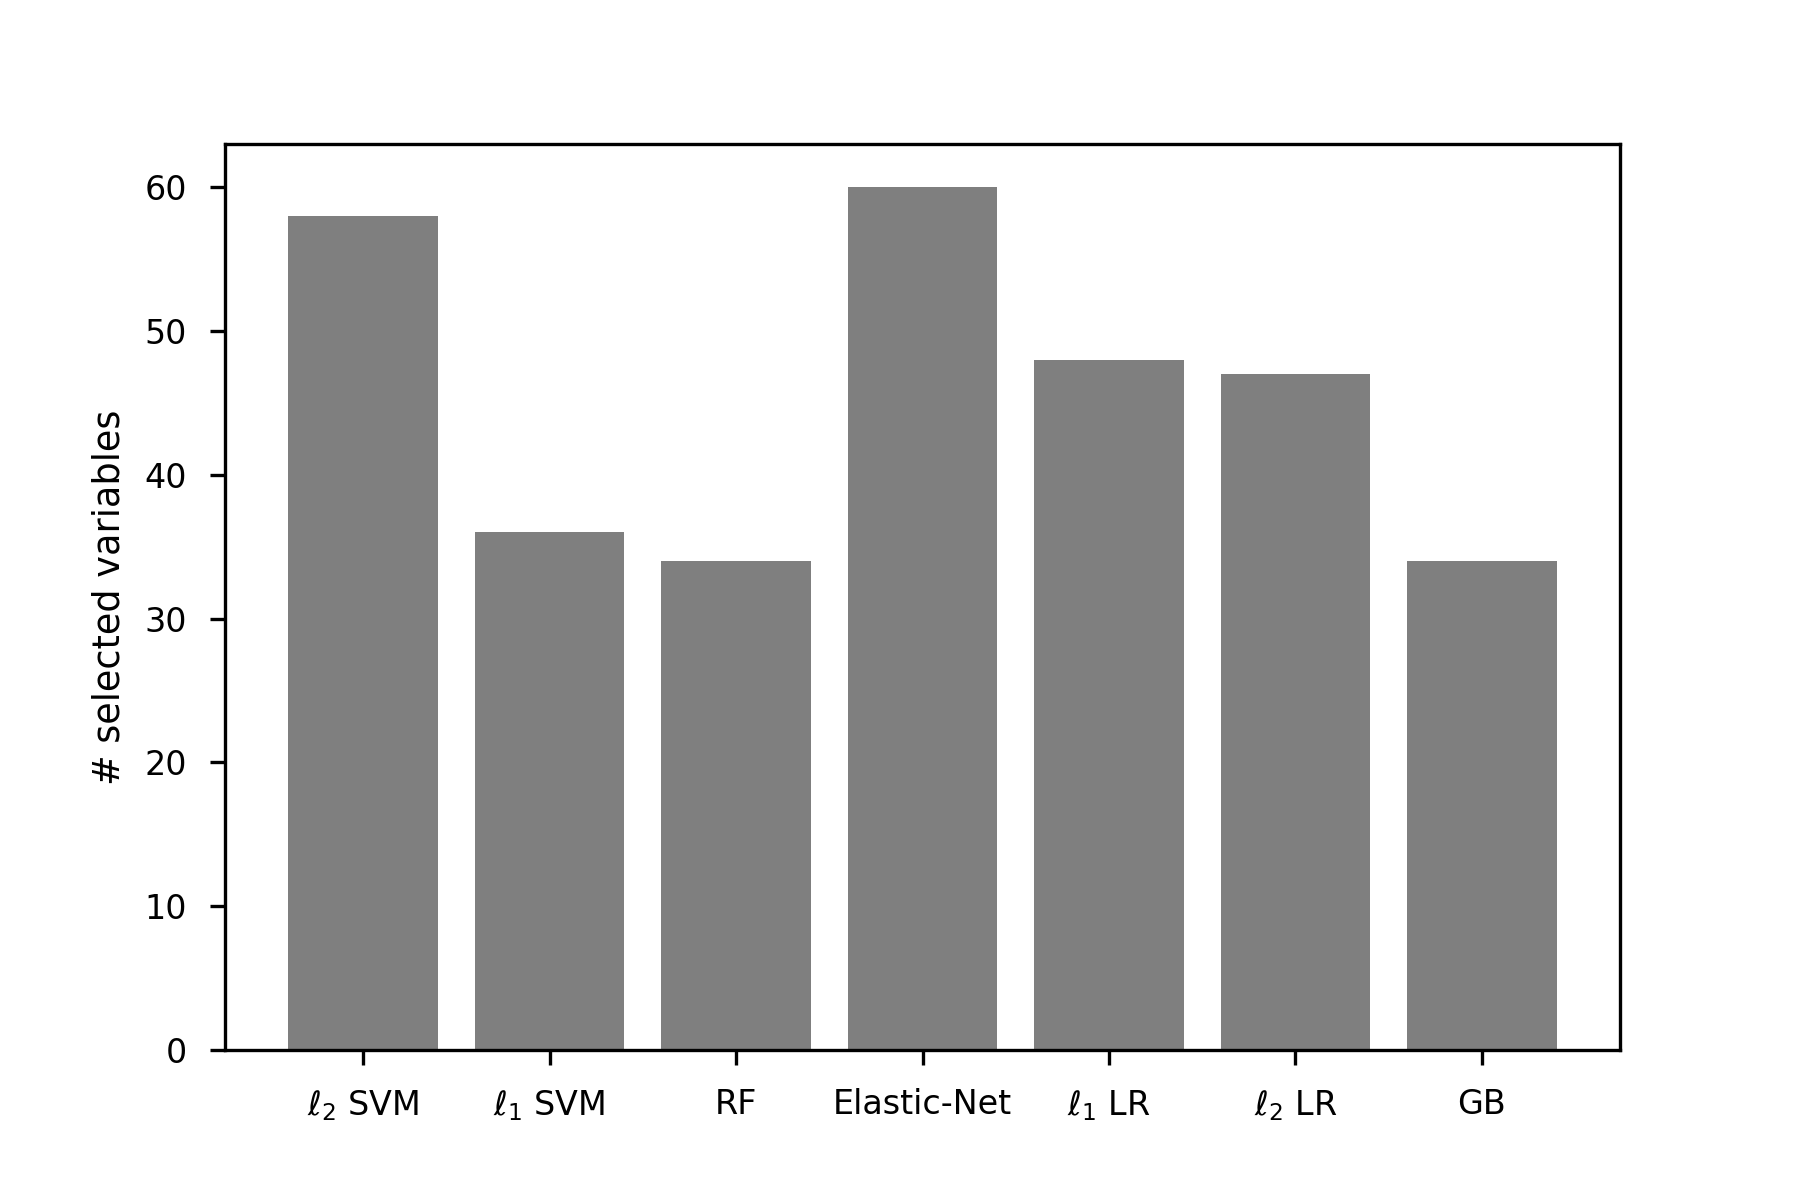
\includegraphics[width=0.8\textwidth]{part2/aism_selected_features.png}
		\caption{The number of variables selected by each of the seven candidate models.} \label{fig:n_selected}
	\end{figure}

	Once refitted on the union of training and validation, but each one considering only the corresponding relevant features, the seven candidate models reach on the test set the performance summarized in Table~\ref{tab:f_final_scores} and visually represented in Figure~\ref{fig:f_final_scores}.
	
	\begin{figure}[]
		\centering
		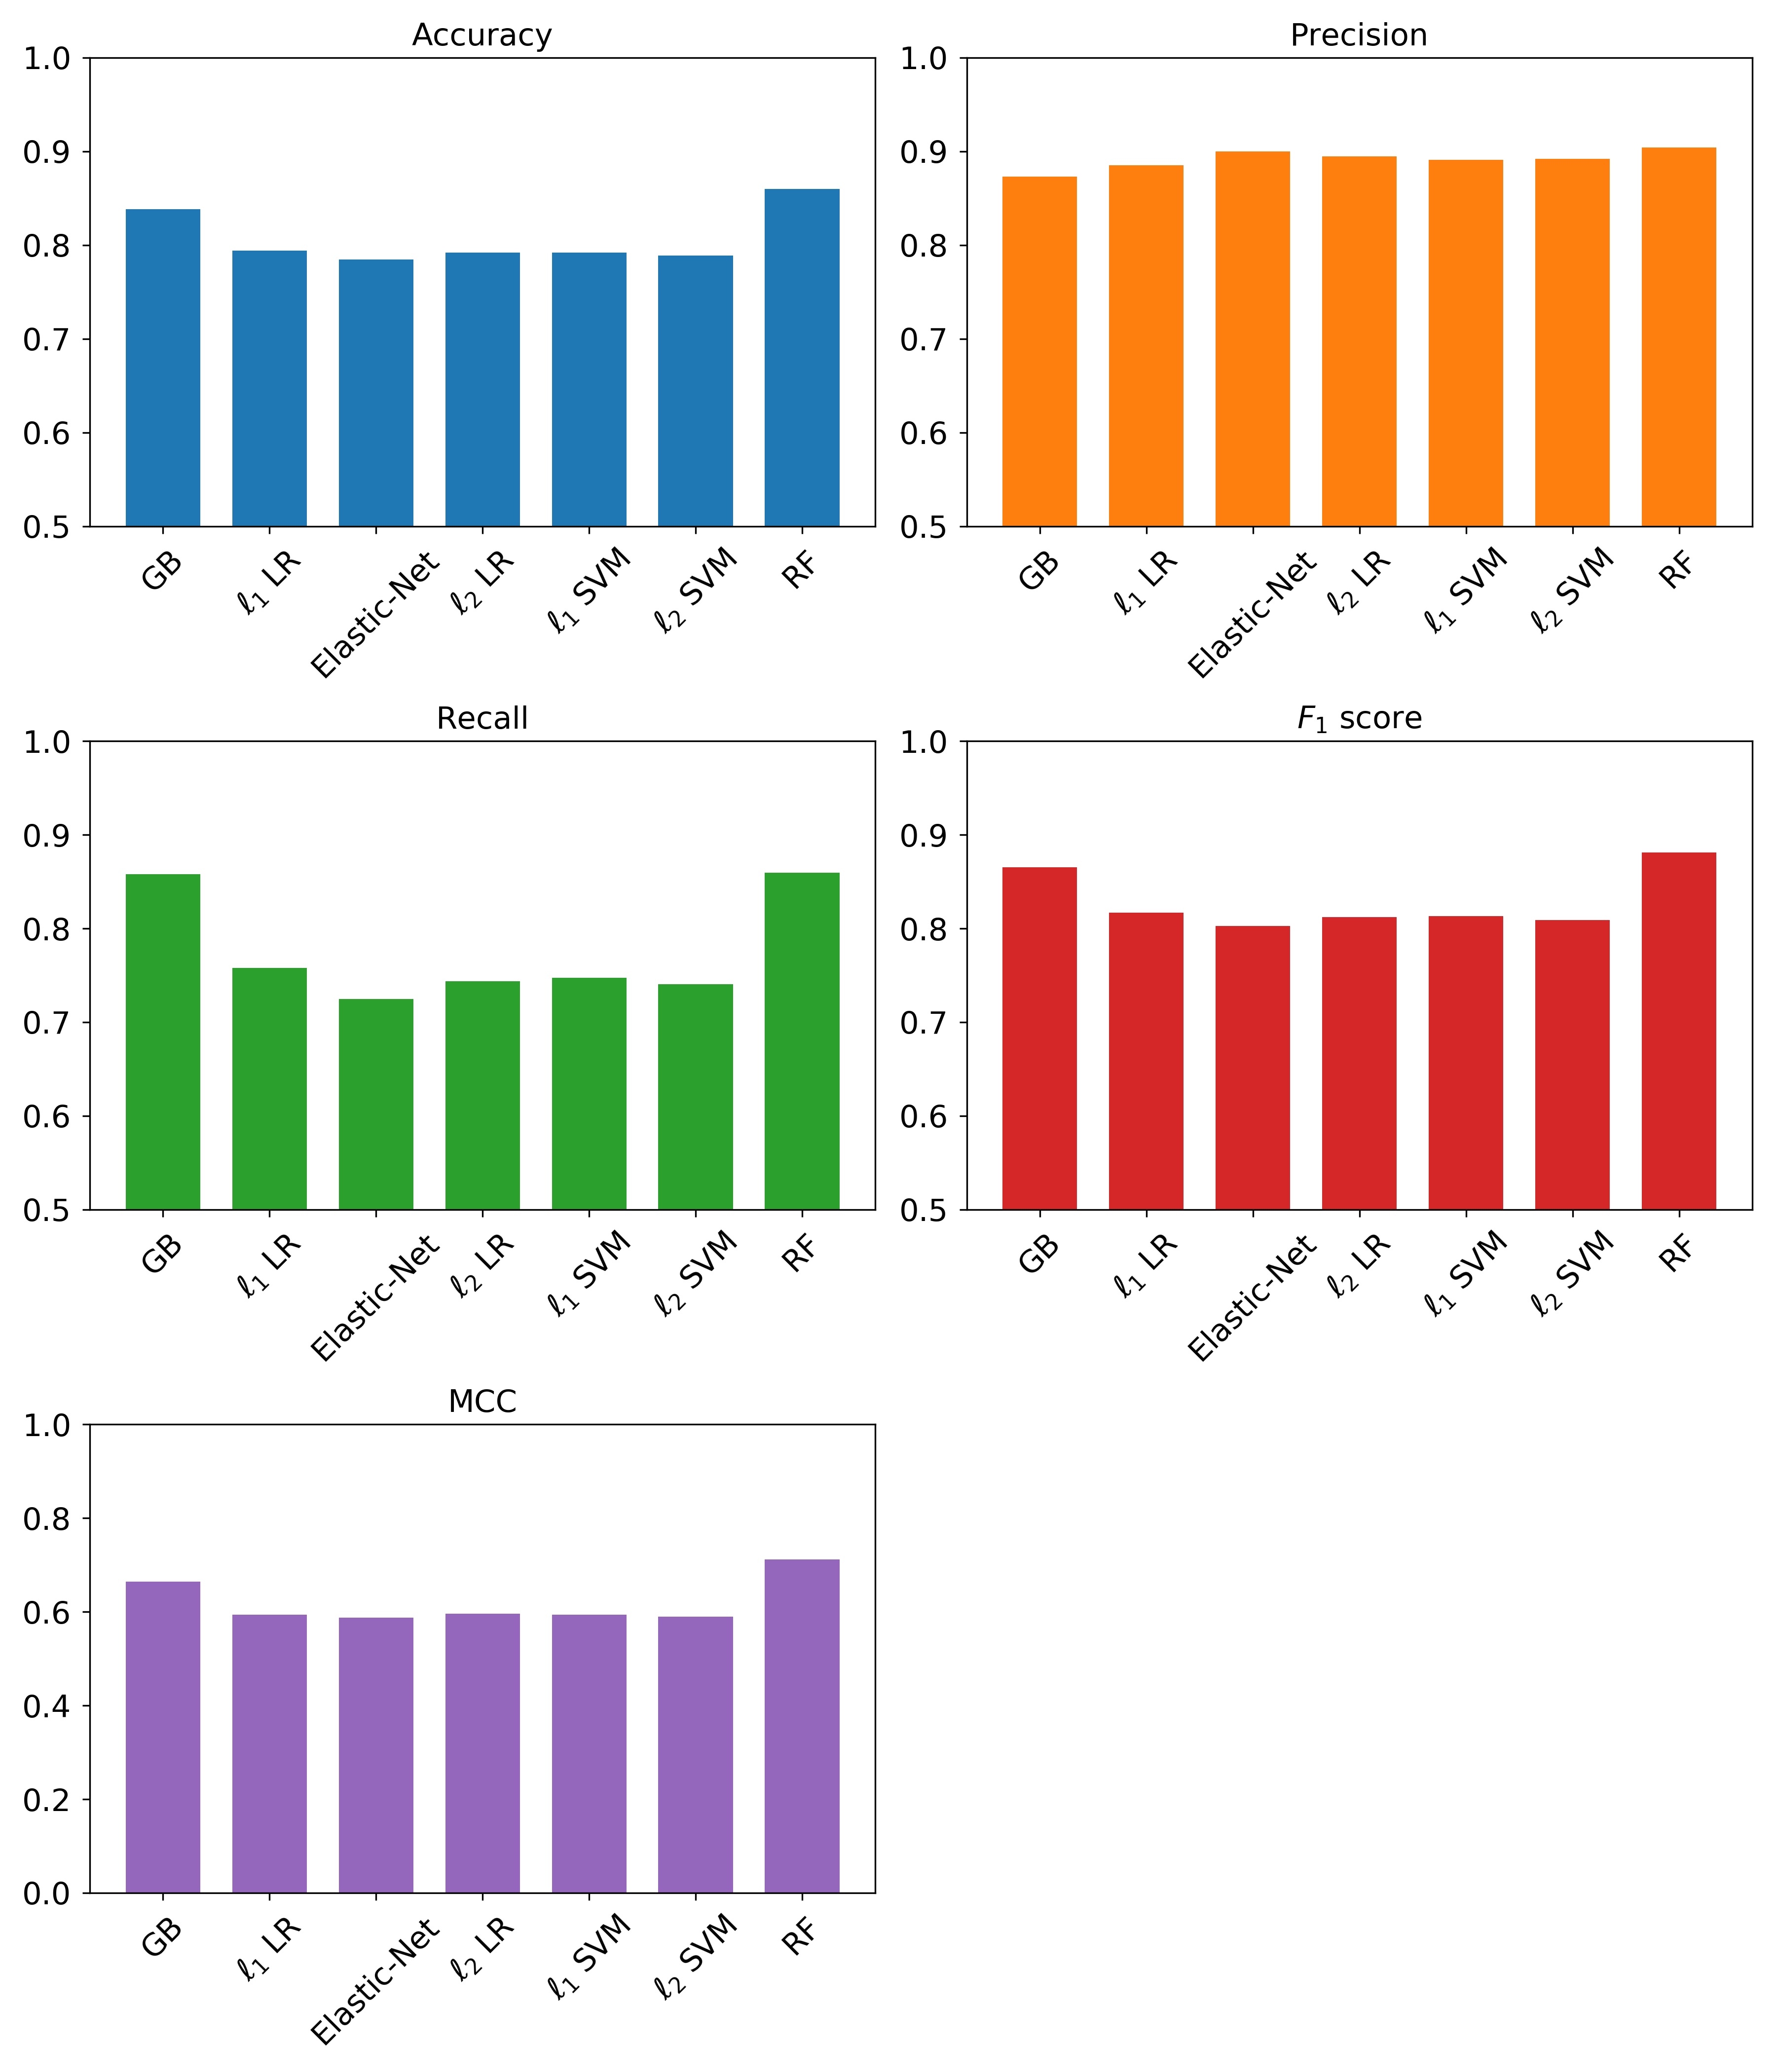
\includegraphics[draft=false, width=0.8\textwidth]{part2/aism_f_final_scores.png}
		\caption{The classification scores achieved by the seven candidate models on the test set.} \label{fig:f_final_scores}
	\end{figure}

	\begin{table}
\centering
\begin{tabular}{lrrrrr}
\toprule
{} &       MCC &  Accuracy &  Precision &    Recall &        F\textsubscript{$1$}-score \\
\midrule
GB      &  0.664097 &  0.838641 &   0.873214 &  0.857895 &  0.865487 \\
RF         &  \textbf{0.711918} &  \textbf{0.859873} &   \textbf{0.904059} &  \textbf{0.859649} &  \textbf{0.881295} \\
Elastic-Net                   &  0.587672 &  0.784501 &   0.899782 &  0.724561 &  0.802721 \\
$\ell_2$ LR &  0.595848 &  0.791932 &   0.894515 &  0.743860 &  0.812261 \\
$\ell_1$ LR &  0.594176 &  0.794055 &   0.885246 &  0.757895 &  0.816635 \\
$\ell_2$ SVM          &  0.589783 &  0.788747 &   0.892178 &  0.740351 &  0.809204 \\
$\ell_1$ SVM          &  0.594076 &  0.791932 &   0.891213 &  0.747368 &  0.812977 \\
\bottomrule
\end{tabular}

\caption{Classification performance scores of the seven candidate models (for the \F problem) achieved on the test set.} \label{tab:f_final_scores}
\end{table}

	
	
	
	
	
	The GB method outperforms the other candidate models reaching accuracy $0.900$, precision $0.936$, recall $0.899$ and $\text{F}_1$ score $0.917$, as shown in  and Figure~\ref{fig:diagnosis_competition}. Therefore we chose it as \F model $\hat{f}(\bm{x})$.
	
	Insights on the use of \PCOs for MS assessment are provided by the sparsity of the \F model induced by the RFE schema.
	The $31$ selected variables are reported in Table~\ref{tab:selected}.
	Comparing the full list of \PCO questionnaires of Table~\ref{tab:proms} with Table~\ref{tab:selected}, we observe that each \PCO used in this study is represented at least once, except \EDINB, and the most represented is \FIM.
	We also see that, whenever possible, the model tends to select aggregate scores (total and subtotal) rather that single items. This is consistent with the clinical practice, where neurologists are more likely to assess patient's health status by using the aggregate scores, rather than the single questions.
	Quite surprisingly, the recent number of relapses is the only additional information not selected by the model.
	Finally, we note that all the domains that are known to be affected by the disease are well covered: mobility (upper and lower limbs), cognition, emotional, fatigue, bladder and psychosocial.
	The heatmap in Figure~\ref{fig:selection_heatmap} shows the Hamming distance estimated across the list of variables selected by the seven \F candidate models. Interestingly, tree-based methods are more prone to select similar variables with respect to linear methods. As expected, the sparsity induced by the $\ell_1$-norm of SLR allows the method to achieve a list of variables similar to the one obtained by SVM-RFE, while the list obtained by ENET includes collinear variables and it is significantly different from the others.
	

	
	
	\item[] \textbf{\G}
	MTEN outperforms the other candidate models in terms of MAE ( $\text{MAE}_{\text{MTEN}}=0.095$, $\text{MAE}_{\text{NNM}}=0.102$, $\text{MAE}_{\text{MLP}}=0.105$), hence we select it as our \G model $\hat{g}(\bm{x})$.
	
	\item[] \textbf{\FOG}
	Finally, the \FOG model $\hat{f} \circ \hat{g}(\bm{x})$, obtained by combining MTEN and GB achieves the following performance scores on the $220$ test samples: accuracy $0.841$, precision $0.900$, recall $0.824$ and $\text{F}_1$ score $0.860$.
	
	
\end{itemize}

 \begin{figure}[]
	\centering
	\subfloat[]{%
		\includegraphics[draft=false, width=0.8\textwidth]{part2/final_scores_2_copy.png}
		\label{fig:diagnosis_competition}%
	}%
	 \hfill%
	\subfloat[]{%
		\includegraphics[draft=false, width=0.8\textwidth]{part2/selection_heatmap_copy.png} \label{fig:selection_heatmap}
	}%
	\caption{A visual representation of the results obtained from the \F model. On the left panel (a) we show the classification performance achieved on the test set by the candidate models. Precision, recall and $\text{F}_1$ score are estimated considering \SP as the positive class. As GB outperforms the other methods on each performance metric, it is chosen as \F model. On the right panel (b) a heatmap displays the distance between the lists of variables selected by each model in terms of their hamming distance. \todo{break figure in two}}\label{fig:f}
\end{figure}





\section{Conclusions and future works}

This chapter describes a temporal model based on \PCOs and ML for disease form prediction in MS.
In particular, we address the tasks of current course assignment, \PCOs evolution prediction and future course assignment. The model is built on a collection of \PCOs acquired on a cohort of individuals enrolled in an ongoing funded study (\textit{DETECT-MS PRO}).

% The measures are categorical or ordinal answers to a given set of \PCOs.
\PCOs data are typically used to corroborate evidence provided by quantitative exams, in our case the absence of clear MS disease form predictors makes the information extracted from \PCOs data the only available resource.
The proposed temporal model was able to correctly assign the current MS form and to foresee future ones with accuracy of $90.0\%$ and $84.1\%$, respectively \todo{fixme}.
This demonstrates that \PCOs can effectively be used as MS disease course predictor.
%In the next future, we plan to expand the data collection with respect to the amount of enrolled subjects as well as the number of time points.

In the next future, we plan to further investigate on the predictive capabilities of the proposed model with longer temporal horizons and to compare it with different approaches, such as probabilistic graphical models.
%, that allow to explicitly incorporate the temporal nature of the data.}

Given the achieved promising results, the proposed model is soon going to be validated in clinical practice, where it will assist the clinicians involved in this study to foresee possible disease course transition and to take important decisions concerning treatment and therapies that can substantially improve the quality of life of their patients.
% In fact, the proposed temporal model was able to correctly foresee the evolution of the disease form of $84.1\%$ of MS patients.

In the context of neurodegenerative diseases, clinicians typically use \PCOs data to corroborate evidences coming from standard quantitative exams \cite{black2013patient}. Interestingly, in our case the absence of clear \SP predictors makes the information extracted from \PCOs data the only available resource.
%Our result shows that a timely prediction of the disease course can be obtained from patient-friendly and low-cost measures.

In the era of precision medicine, the problem of predicting MS course evolution still relies on stressful exams and clinical judgement.
To the best of our knowledge, this is the first attempt to solve this delicate task leveraging only on patient-friendly measures and ML.


